% Soubory musí být v kódování, které je nastaveno v příkazu \usepackage[...]{inputenc}

\documentclass[%        Základní nastavení
%  draft,    				  % Testovací překlad
  12pt,       				% Velikost základního písma je 12 bodů
  a4paper,    				% Formát papíru je A4
  oneside,      			% Jednostranný tisk
	%twoside,      			% Dvoustranný tisk (kapitoly a další důležité části tedy začínají na lichých stranách)
	unicode,						% Záložky a metainformace ve výsledném  PDF budou v kódování unicode
]{report}				    	% Dokument třídy 'zpráva', vhodná pro sazbu závěrečných prací s kapitolami

\usepackage[utf8]		  %	Kódování zdrojových souborů je UTF-8
	{inputenc}					% Balíček pro nastavení kódování zdrojových souborů

\usepackage[				% Nastavení geometrie stránky
	bindingoffset=10mm,		% Hřbet pro vazbu
	hmargin={25mm,25mm},	% Vnitřní a vnější okraj  (jsou nehezky shodné; jakási úroveň estetiky je dosažena pomocí hřbetu)
	vmargin={25mm,34mm},	% Horní a dolní okraj
	footskip=17mm,			  % Velikost zápatí
	nohead,					      % Bez záhlaví
	marginparsep=2mm,		  % Vzdálenost marginálií
	marginparwidth=18mm,	% Šířka marginálií
]{geometry}

\usepackage{sectsty}
	%přetypuje nadpisy všech úrovní na bezpatkové, kromě \chapter, která je přenastavena zvlášť v thesis.sty
	\allsectionsfont{\sffamily}

\usepackage{graphicx} % Balíček 'graphicx' pro vkládání obrázků
											% Nutné pro vložení logotypů školy a fakulty
\usepackage{tikz}
\usetikzlibrary{shapes,arrows,positioning}

\usepackage{float}

\usepackage[          % Balíček 'acronym' pro sazby zkratek a symbolů
	nohyperlinks				% Nebudou tvořeny hypertextové odkazy do seznamu zkratek
]{acronym}						
											% Nutné pro použití prostředí 'acronym' balíčku 'thesis'

\usepackage[
	breaklinks=true,		% Hypertextové odkazy mohou obsahovat zalomení řádku
	hypertexnames=false % Názvy hypertext. odkazů budou tvořeny nezávisle na názvech TeXu
]{hyperref}						% Balíček 'hyperref' pro sazbu hypertextových odkazů
											% Nutné pro použití příkazu 'pdfsettings' balíčku 'thesis'

\usepackage{pdfpages} % Balíček umožňující vkládat stránky z PDF souborů
                      % Nutné při vkládání titulních listů a zadání přímo
                      % ve formátu PDF z informačního systému

\usepackage{enumitem} % Balíček pro nastavení mezerování v odrážkách
  \setlist{topsep=0pt,partopsep=0pt,noitemsep} % konkrétní nastavení

\usepackage{cmap} 		% Balíček cmap zajišťuje, že PDF vytvořené `pdflatexem' je
											% plně "prohledávatelné" a "kopírovatelné"

%\usepackage{upgreek}	% Balíček pro sazbu stojatých řeckých písmem
											%% např. stojaté pí: \uppi
											%% např. stojaté mí: \upmu (použitelné třeba v mikrometrech)
											%% pozor, grafická nekompatibilita s fonty typu Computer Modern!
                      
\usepackage{amsmath} %balíček pro sabu náročnější matematiky                 

\usepackage{dirtree}	% sazba adresářové struktury
                      % vhodné pro prezentaci obsahu elektronické přílohy (např. CD)

\usepackage[formats]{listings}	% Balíček pro sazbu zdrojových textů
\lstset{              % nastavení
%	Definice jazyka použitého ve výpisech
%    language=[LaTeX]{TeX},	% LaTeX
%	language={Matlab},		% Matlab
	language={C},           % jazyk C
    basicstyle=\ttfamily,	% definice základního stylu písma
    tabsize=2,			% definice velikosti tabulátoru
    inputencoding=utf8,         % pro soubory uložené v kódování UTF-8
		columns=fixed,  %fixed nebo flexible,
		fontadjust=true %licovani sloupcu
    extendedchars=true,
    literate=%  definice symbolů s diakritikou
    {á}{{\'a}}1
    {ä}{{\"a}}1
    {č}{{\v{c}}}1
    {ď}{{\v{d}}}1
    {é}{{\'e}}1
    {ě}{{\v{e}}}1
    {í}{{\'i}}1
    {ň}{{\v{n}}}1
    {ó}{{\'o}}1
    {ô}{{\^o}}1
    {ř}{{\v{r}}}1
    {š}{{\v{s}}}1
    {ť}{{\v{t}}}1
    {ú}{{\'u}}1
    {ů}{{\r{u}}}1
    {ý}{{\'y}}1
    {ž}{{\v{z}}}1
    {Á}{{\'A}}1
    {Č}{{\v{C}}}1
    {Ď}{{\v{D}}}1
    {É}{{\'E}}1
    {Ě}{{\v{E}}}1
    {Í}{{\'I}}1
    {Ň}{{\v{N}}}1
    {Ó}{{\'O}}1
    {Ř}{{\v{R}}}1
    {Š}{{\v{S}}}1
    {Ť}{{\v{T}}}1
    {Ú}{{\'U}}1
    {Ů}{{\r{U}}}1
    {Ý}{{\'Y}}1
    {Ž}{{\v{Z}}}1
}

%%%%%%%%%%%%%%%%%%%%%%%%%%%%%%%%%%%%%%%%%%%%%%%%%%%%%%%%%%%%%%%%%
%%%%%%      Definice informací o dokumentu             %%%%%%%%%%
%%%%%%%%%%%%%%%%%%%%%%%%%%%%%%%%%%%%%%%%%%%%%%%%%%%%%%%%%%%%%%%%%

% V tomto souboru se nastavují téměř veškeré informace, proměnné mezi studenty:
% jméno, název práce, pohlaví atd.
% Tento soubor je SDÍLENÝ mezi textem práce a prezentací k obhajobě -- netřeba něco nastavovat na dvou místech.

\usepackage[
%%% Z následujících voleb jazyka lze použít pouze jednu
  %czech-english,		% originální jazyk je čeština, překlad je anglicky (výchozí)
  %english-czech,	% originální jazyk je angličtina, překlad je česky
  slovak-english,	% originální jazyk je slovenština, překlad je anglicky
  %english-slovak,	% originální jazyk je angličtina, překlad je slovensky
%
%%% Z následujících voleb typu práce lze použít pouze jednu
  semestral,		  % semestrální práce (výchozí)
  %bachelor,			%	bakalářská práce
  %master,			  % diplomová práce
  %treatise,			% pojednání o disertační práci
  %doctoral,			% disertační práce
%
%%% Z následujících voleb zarovnání objektů lze použít pouze jednu
%  left,				  % rovnice a popisky plovoucích objektů budou zarovnány vlevo
	center,			    % rovnice a popisky plovoucích objektů budou zarovnány na střed (vychozi)
%
]{thesis}   % Balíček pro sazbu studentských prací


%%% Jméno a příjmení autora ve tvaru
%  [tituly před jménem]{Křestní}{Příjmení}[tituly za jménem]
% Pokud osoba nemá titul před/za jménem, smažte celý řetězec '[...]'
\author[Bc.]{Jakub}{Franka}

%%% Identifikační číslo autora (VUT ID)
\butid{220976}

%%% Pohlaví autora/autorky
% (nepoužije se ve variantě english-czech ani english-slovak)
% Číselná hodnota: 1...žena, 0...muž
\gender{0}

%%% Jméno a příjmení vedoucího/školitele včetně titulů
%  [tituly před jménem]{Křestní}{Příjmení}[tituly za jménem]
% Pokud osoba nemá titul před/za jménem, smažte celý řetězec '[...]'
\advisor[Ing.]{Ilona}{Janáaková}[Ph.D.]

%%% Jméno a příjmení oponenta včetně titulů
%  [tituly před jménem]{Křestní}{Příjmení}[tituly za jménem]
% Pokud osoba nemá titul před/za jménem, smažte celý řetězec '[...]'
% Nastavení oponenta se uplatní pouze v prezentaci k obhajobě;
% v případě, že nechcete, aby se na titulním snímku prezentace zobrazoval oponent, pouze příkaz zakomentujte;
% u obhajoby semestrální práce se oponent nezobrazuje (jelikož neexistuje)
% U dizertační práce jsou typicky dva až tři oponenti. Pokud je chcete mít na titulním slajdu, prosím ručně odkomentujte a upravte jejich jména v definici "VUT title page" v souboru thesis.sty.
\opponent[doc.\ Mgr.]{Křestní}{Příjmení}[Ph.D.]

%%% Název práce
%  Parametr ve složených závorkách {} je název v originálním jazyce,
%  parametr v hranatých závorkách [] je překlad (podle toho jaký je originální jazyk).
%  V případě, že název Vaší práce je dlouhý a nevleze se celý do zápatí prezentace, použijte příkaz
%  \def\insertshorttitle{Zkác.\ náz.\ práce}
%  kde jako parametr vyplníte zkrácený název. Pokud nechcete zkracovat název, budete muset předefinovat,
%  jak se vytváří patička slidu. Viz odkaz: https://bit.ly/3EJTp5A
\title[System for tracking and classification of objects in the sky]{Systém pro sledování a klasifikaci objektů na obloze}

%%% Označení oboru studia
%  Parametr ve složených závorkách {} je název oboru v originálním jazyce,
%  parametr v hranatých závorkách [] je překlad
\specialization[Cybernetics, automation and measurement]{Kybernetika, automatizace a měření}

%%% Označení ústavu
%  Parametr ve složených závorkách {} je název ústavu v originálním jazyce,
%  parametr v hranatých závorkách [] je překlad
\department[Department of Control and Instrumentation]{Ústav automatizace a měřicí techniky}
%\department[Department of Biomedical Engineering]{Ústav biomedicínského inženýrství}
%\department[Department of Electrical Power Engineering]{Ústav elektroenergetiky}
%\department[Department of Electrical and Electronic Technology]{Ústav elektrotechnologie}
%\department[Department of Physics]{Ústav fyziky}
%\department[Department of Foreign Languages]{Ústav jazyků}
%\department[Department of Mathematics]{Ústav matematiky}
%\department[Department of Microelectronics]{Ústav mikroelektroniky}
%\department[Department of Radio Electronics]{Ústav radioelektroniky}
%\department[Department of Theoretical and Experimental Electrical Engineering]{Ústav teoretické a experimentální elektrotechniky}
%\department[Department of Telecommunications]{Ústav telekomunikací}
%\department[Department of Power Electrical and Electronic Engineering]{Ústav výkonové elektrotechniky a elektroniky}

%%% Označení fakulty
%  Parametr ve složených závorkách {} je název fakulty v originálním jazyce,
%  parametr v hranatých závorkách [] je překlad
%\faculty[Faculty of Architecture]{Fakulta architektury}
\faculty[Faculty of Electrical Engineering and~Communication]{Fakulta elektrotechniky a~komunikačních technologií}
%\faculty[Faculty of Chemistry]{Fakulta chemická}
%\faculty[Faculty of Information Technology]{Fakulta informačních technologií}
%\faculty[Faculty of Business and Management]{Fakulta podnikatelská}
%\faculty[Faculty of Civil Engineering]{Fakulta stavební}
%\faculty[Faculty of Mechanical Engineering]{Fakulta strojního inženýrství}
%\faculty[Faculty of Fine Arts]{Fakulta výtvarných umění}
%
%Nastavení logotypu (v hranatych zavorkach zkracene logo, ve slozenych plne):
\facultylogo[logo/FEKT_zkratka_barevne_PANTONE_CZ]{logo/UTKO_color_PANTONE_CZ}

%%% Rok odevzdání práce
\graduateyear{2024}
%%% Akademický rok odevzdání práce
\academicyear{2023/24}

%%% Datum obhajoby (uplatní se pouze v prezentaci k obhajobě)
\date{11.\,11.\,1980} 

%%% Místo obhajoby
% Na titulních stránkách bude automaticky vysázeno VELKÝMI písmeny (pokud tyto stránky sází šablona)
\city{Brno}

%%% Abstrakt
\abstract[%
Překlad abstraktu
(v~angličtině, pokud je originálním jazykem čeština či slovenština; v~češtině či slovenštině, pokud je originálním jazykem angličtina)
]{%
Abstrakt práce v~originálním jazyce
}

%%% Klíčová slova
\keywrds[%
Překlad klíčových slov
(v~angličtině, pokud je originálním jazykem čeština či slovenština; v~češtině či slovenštině, pokud je originálním jazykem angličtina)
]{%
Klíčová slova v~originálním jazyce
}

%%% Poděkování
\acknowledgement{%
Rád bych poděkoval vedoucímu bakalářské/diplomové/disertační práce
panu Ing.~XXX YYY, Ph.D.\ za odborné vedení,
konzultace, trpělivost a~podnětné návrhy k~práci.
}%  % do tohoto souboru doplňte údaje o sobě, druhu práce, názvu...

%%%%%%%%%%%%%%%%%%%%%%%%%%%%%%%%%%%%%%%%%%%%%%%%%%%%%%%%%%%%%%%%%%%%%%%%

%%%%%%%%%%%%%%%%%%%%%%%%%%%%%%%%%%%%%%%%%%%%%%%%%%%%%%%%%%%%%%%%%%%%%%%%
%%%%%%     Nastavení polí ve Vlastnostech dokumentu PDF      %%%%%%%%%%%
%%%%%%%%%%%%%%%%%%%%%%%%%%%%%%%%%%%%%%%%%%%%%%%%%%%%%%%%%%%%%%%%%%%%%%%%
%% Při načteném balíčku 'hyperref' lze použít příkaz '\pdfsettings':
\pdfsettings
%  Nastavení polí je možné provést také ručně příkazem:
%\hypersetup{
%  pdftitle={Název studentské práce},    	% Pole 'Document Title'
%  pdfauthor={Autor studenstké práce},   	% Pole 'Author'
%  pdfsubject={Typ práce}, 						  	% Pole 'Subject'
%  pdfkeywords={Klíčová slova}           	% Pole 'Keywords'
%}
%%%%%%%%%%%%%%%%%%%%%%%%%%%%%%%%%%%%%%%%%%%%%%%%%%%%%%%%%%%%%%%%%%%%%%%

\pdfmapfile{=vafle.map}

%%%%%%%%%%%%%%%%%%%%%%%%%%%%%%%%%%%%%%%%%%%%%%%%%%%%%%%%%%%%%%%%%%%%%%%
%%%%%%%%%%%       Začátek dokumentu               %%%%%%%%%%%%%%%%%%%%%
%%%%%%%%%%%%%%%%%%%%%%%%%%%%%%%%%%%%%%%%%%%%%%%%%%%%%%%%%%%%%%%%%%%%%%%
\begin{document}
\pagestyle{empty} %vypnutí číslování stránek

%%% Vložení desek -- od září 2021 na žádost fakulty nepoužíváno
%\includepdf[pages=1]%  buďto generovaných informačním systémem
  %{pdf/student-desky}% název souboru nesmí obsahovat mezery!
%%% NEBO vytvoření desek z balíčku
%%\makecover
%%%
%\oddpage % při dvojstranném tisku přidá prázdnou stránku
%% kazdopádně ale:
%\setcounter{page}{1} %resetovaní čítače stránek -- desky do číslování nezahrnujeme

%% Vložení titulního listu
\includepdf[pages=1]%    buďto generovaného informačním systémem
  {pdf/student-titulka}% název souboru nesmí obsahovat mezery!
%% NEBO vytvoření titulní stránky z balíčku
%\maketitle
%%
\oddpage  % při dvojstranném tisku se přidá prázdná stránka
   
%% Vložení zadání
\includepdf[pages=1]%   buďto generovaného informačním systémem
  {pdf/student-zadani}% název souboru nesmí obsahovat mezery!
%% NEBO lze vytvořit prázdný list příkazem ze šablony
%\patternpage{}%
%	{\sffamily\Huge\centering ZDE VLOŽIT LIST ZADÁNÍ}%
%	{\sffamily\centering Z~důvodu správného číslování stránek}
%%
\oddpage% při dvojstranném tisku se přidá prázdná stránka

%% Vysázení stránky s abstraktem
\makeabstract

% Vysázení stránky s rozšířeným abstraktem
% (pokud píšete práci v češtině či slovenštině, vložení rozšířeného abstraktu zrušte;
%  pro semestrální projekt také není potřeba rozšířený abstrakt uvádět)
% Vysázení stránky s rozšířeným abstraktem
% (týká se pouze bc. a dp. prací psaných v angličtině, viz Směrnice rektora 72/2017)
\cleardoublepage
\noindent
{\large\sffamily\bfseries\MakeUppercase{Rozšířený abstrakt}}
\\
Výtah ze směrnice rektora 72/2017:\\
\emph{Bakalářská a diplomová práce předložená v angličtině musí obsahovat rozšířený abstrakt v češtině
nebo slovenštině (čl. 15). To se netýká studentů, kteří studují studijní program akreditovaný v
angličtině.}
(čl. 3, par. 7)\\
\emph{Nebude-li vnitřní normou stanoveno jinak, doporučuje se rozšířený abstrakt o rozsahu přibližně 3
normostrany, který bude obsahovat úvod, popis řešení a shrnutí a~zhodnocení výsledků.}
(čl. 15, par. 5)

%%% Vysázení citace práce
\makecitation

%%% Vysázení prohlášení o samostatnosti
\makedeclaration

%%% Vysázení poděkování
\makeacknowledgement

%%% Vysázení obsahu
\tableofcontents

%%% Vysázení seznamu obrázků
% (vynechejte, pokud máte dva nebo méně obrázků)
\listoffigures

%%% Vysázení seznamu tabulek
% (vynechejte, pokud máte dvě nebo méně tabulek)
\listoftables

%%% Vysázení seznamu výpisů kódu
% (vynechejte, pokud máte dva nebo méně výpisů)
\lstlistoflistings

\cleardoublepage\pagestyle{plain}   % zapnutí číslování stránek

%Pro vkládání kapitol i příloh používejte raději \include než \input
%%% Vložení souboru 'text/uvod.tex' s úvodem
\chapter*{Úvod}
\phantomsection
\addcontentsline{toc}{chapter}{Úvod}

V~súčasnej dobe hrá počítačové videnie dôležitú rolu v~mnohých aplikáciách. Táto práca sa~zameriava na~jeho využitie pri~návrhu systému schopného detekovať, trasovať a~klasifikovať objekty lietajúce na~oblohe. Cieľom je vytvoriť robustný systém schopný nasadenia v~reálnych nepriaznivých podmienkach so~schopnosťou detekcie a~klasifikácie rôznych typov živých aj~umelo vytvorených lietajúcich objektov. Je požadovaná možnosť použitia rôznych prístupov spracovania vstupných dát a~porovnanie ich výkonu a~presnosti. Pri návrhu systému je nutné zvážiť obmedzený výkon výpočtovej jednotky systému a~voliť jednoduchšie.

Systém bude získavať obrazové dáta pomocou statickej kamery sledujúcej časť oblohy. Časť obrazu môže obsahovať aj~horizont. Kamera v~bude reálnom čase zachytávať sekvenciu snímkov. Na~nich systém musí rozpoznať pohybujúce sa~objekty na~pozadí, ktoré sa~môže s~postupom času tiež pohybovať či~meniť, či~už~kvôli pohybujúcim oblakom alebo zmene svetelných podmienok.

Detekované objekty budú klasifikované do~piatich tried: vták, hmyz, lietadlo, helikoptéra, dron. Kvôli rôznym farbám rôznych inštancii týchto objektov môžu mať objekty vyšší, ale~aj~nižší jas ako~pozadie.

Táto práca bude postupovať od~teoretických základov do~konkrétneho návrhu a~implementácie popísaného systému počítačového videnia.

Prvá kapitola sa~venuje základným princípom detekcie objektov v~obraze. Sú tu~preskúmané existujúce metódy s~porovnaním ich~výhod a~nevýhod, čo~povedie k~výberu vhodných metód pre~navrhovaný systém.

V~druhej kapitole bude popísané získavanie charakteristík popisujúcich jednotlivé detekované objekty. Zohľadňujú sa~tu~aspekty ako~tvar, farba a~ďalšie príznaky, na~ktorých záleží klasifikácia v~ďalšom kroku.

Na~základe popisu objektov bude v~ďalšej kapitole popísaná problematika klasifikácie, teda rozpoznávania a~zaradenia detekovaných objektov do~definovaných tried podľa ich~typu (lietadlo, helikoptéra, vták, hmyz, \dots).

Štvrtá kapitola predstaví moderné metódy integrujúce detekciu a~klasifikáciu do~jedného procesu. Cieľom je optimalizácia efektivity a~jednoduchosti architektúry systému.

Následne bude navrhnutý a~odôvodnený výber hardvérových komponentov systému. Budú porovnané mikropočítače vhodné na~aplikáciu v~tejto práci a~zvolené vhodné periférie na~získavanie dát a~užívateľské rozhranie.

Pre správne naučenie modelov použitých v~systéme je nevyhnutné vytvoriť dostatočne rozsiahlu a~správne navrhnutú anotovanú množinu dát, v~prípade algoritmov počítačového videnia ide o~databázu snímkov s~označenými a~triedenými objektami. Šiesta kapitola sa~zameriava na~tvorbu tejto databázy (datasetu) a~jej~validáciu.

V~poslednej kapitole bude zdokumentovaný návrh softvéru pre~systém detekcie, klasifikácie a~trasovania objektov. V~tejto kapitole bude priblížená štruktúra aplikácie, nástroje použité pri~vývoji a~návrh jej~užívateľského rozhrania.

% Úvod studentské práce, např\,\dots
% 
% Nečíslovaná kapitola Úvod obsahuje \uv{seznámení} čtenáře s~problematikou práce.
% Typicky se zde uvádí:
% (a) do jaké tematické oblasti práce spadá, (b) co jsou hlavní cíle celé práce a (c) jakým způsobem jich bylo dosaženo.
% Úvod zpravidla nepřesahuje jednu stranu.
% Poslední odstavec Úvodu standardně představuje základní strukturu celého dokumentu.
% 
% Tato práce se věnuje oblasti \acs{DSP} (\acl{DSP}), zejména jevům, které nastanou při nedodržení Nyquistovy podmínky pro \ac{symfvz}.%
% \footnote{Tato věta je pouze ukázkou použití příkazů pro sazbu zkratek.}
% 
% Šablona je nastavena na \emph{dvoustranný tisk}.
% Nebuďte překvapeni, že ve vzniklém PDF jsou volné stránky.
% Je to proto, aby důležité stránky jako např.\ začátky kapitol začínaly po vytisknutí a svázání vždy na pravé straně.
% %
% Pokud máte nějaký závažný důvod sázet (a~zejména tisknout) jednostranně, nezapomeňte si přepnout volbu \texttt{twoside} na \texttt{oneside}!

%%% Vložení souboru 'text/cile.tex' s úvodem
% \chapter*{Cíle práce}
% \phantomsection
% \addcontentsline{toc}{chapter}{Cíle práce}
% 
% Konkrétní specifikace cílů, které má autor v~práci vyřešit.
% Tato kapitola je \emph{volitelná} -- pokud váš studijní program nevyžaduje zvláštní kapitolu s cíli,
% cíle specifikujte v~rámci Úvodu.

%%% Vložení souboru 'text/reseni' s popisem řešení práce
% (rozdělte na více souborů či kapitol, pokud je vhodné)
\chapter{Detekcia objektov v obraze}

    Pre niektoré techniky klasifikácie objektov je nutné najprv v obraze tieto objekty nájsť. Existuje k tomu veľké množstvo metodík, pri čom každá z nich má svoje výhody a nevýody. Je teda nutnosťou zistiť ktorá metóda najviac vyhovuje použitiu pre túto prácu.

\section{Prahovanie}

    Prahovanie je jasová transformácia pri ktorej je šedotónový obraz rozdelený na dve a viac oblastí podľa jasovej úrovne pixelov. O tom, do ktorej z oblastí je daný pixel priradený rozhoduje prah, ktorého hodnotu je treba určiť. Výsledkom je obraz s len dvomi úrovňami jasu - binárny obraz.

    Pri správnom predspracovaní obrazu prahovaním, je možné v ňom jednoducho oddeliť objekty od pozadia, v prípade ak sa jas objektu dostatočne lýši od jasu pozadia. Ak sa však jasové hodnoty objektu a pozadia príliš podobajú, nemusí existovať dostatočne robustné určenie prahu oddeľujúceho objekty od pozadia.

    \begin{figure}[!ht]
        \begin{center}
            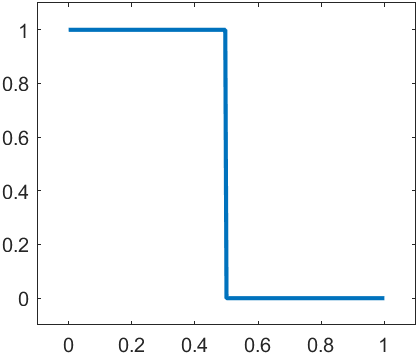
\includegraphics[scale=.4]{obrazky/threshold/thresholding.png}
        \end{center}
        \caption{Funkcia prahovania s prahom 0.5 pre svetlé pozadie}
    \end{figure}

\subsection{Globálne prahovanie}

    Globálne prahovanie je často používaná technika pri ktorej je použítý jediný prah na celý obraz, čo nemusí byť vhodné v prípade ak je jasová úroveň pozadia rôzna v rôznych miestach obrazu.

    \begin{itemize}
        \item \textbf{Jednoduché prahovanie} je technika pri ktorej je globálny prah určený dopredu ručne. V prípade že sa jasová úroveň pozadia v čase mení, je vhodnejšie použiť techniky s adaptívnym nastavením prahu.

        \item Prahovanie \textbf{podľa známeho rozloženia} predpokladá že poznáme relatívnu veľkosť oblasti ktorú zaberá pozadie v obraze. Ak vieme že objekt je svetlejší ako pozadie, môžeme určiť prah z kumulatívneho histogramu tak, aby relatívny počet pixelov pod úrovňou prahu bol rovnaký ako oblasť ktorú ma zaberať pozadie.

        \item Algoritmus \textbf{K-Means} (K priemerov) pre zhlukovú analýzu, rozdeľuje dáta do skupín s cieľom minimalizovať vzdialenosť bodov v zhluku a maximalizovať vzdialenosť medzi zhlukmi. Jedná sa o algorytmus učenia bez učiteľa. Funguje na princípe iterovaného posúvania \emph{k} stredov zhlukov (v prípade binárneho prahovania je \emph{k = 2}), smerom k priemeru hodnôt priradenému danému stredu v aktuálnom kroku.

        \item \textbf{Otsuova metóda} automatického určenia prahu je založená na maximalizovaní vzájomnej odchýlky medzi triedami. Využíva normalizovaný kumulatívny histogram z ktorého určuje vzájomnú rozptyl pre všetky možné hodnoty prahu a vyberá ten optimálny. 
    \end{itemize}

    \begin{figure}[!ht]
        \centering
        \begin{tikzpicture}[>=stealth, node distance=5cm]
            \node (image1) {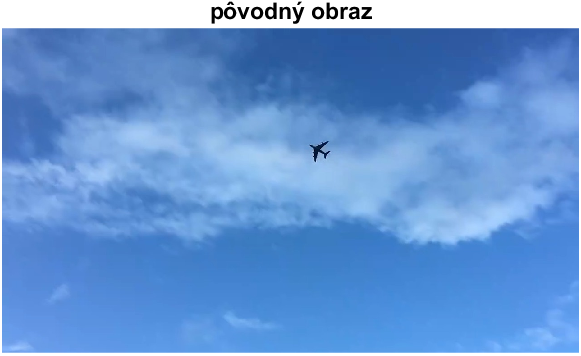
\includegraphics[width=.3\textwidth]{obrazky/threshold/img.png}};
            \node (image2) [right of=image1] {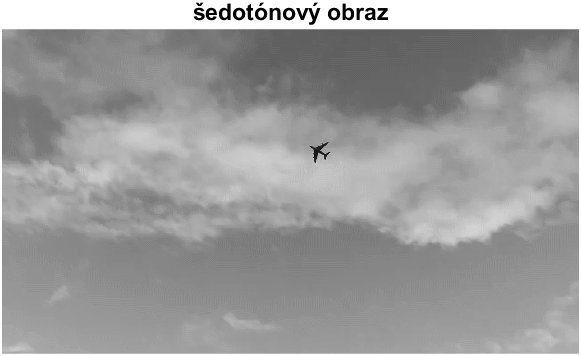
\includegraphics[width=.3\textwidth]{obrazky/threshold/img_gray.png}};
            \node (image3) [right of=image2] {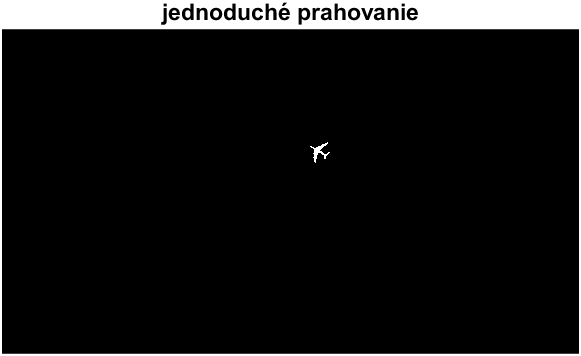
\includegraphics[width=.3\textwidth]{obrazky/threshold/img_simple_thresh.png}};

            \draw[->] (image1) -- (image2) node[midway, above] {};
            \draw[->] (image2) -- (image3) node[midway, above] {};
        \end{tikzpicture}
        \begin{tikzpicture}[>=stealth, node distance=5cm]
            \node (image1) {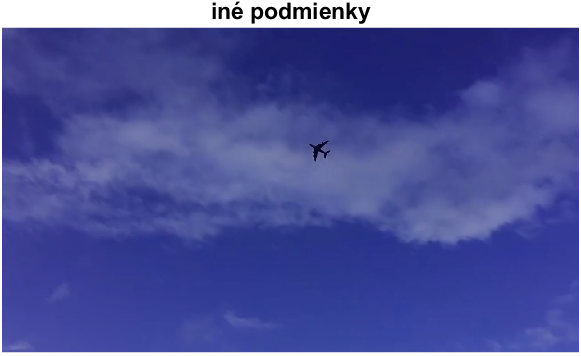
\includegraphics[width=.3\textwidth]{obrazky/threshold/img_dark.png}};
            \node (image2) [right of=image1] {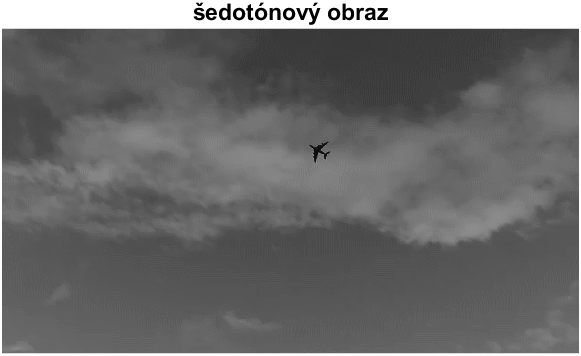
\includegraphics[width=.3\textwidth]{obrazky/threshold/img_dark_gray.png}};
            \node (image3) [right of=image2] {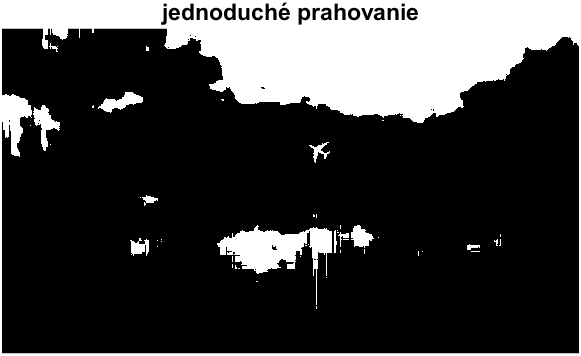
\includegraphics[width=.3\textwidth]{obrazky/threshold/img_dark_simple_thresh.png}};

            \draw[->] (image1) -- (image2) node[midway, above] {};
            \draw[->] (image2) -- (image3) node[midway, above] {};
        \end{tikzpicture}
        \caption{Jednoduché prahovanie}
    \end{figure}

    \begin{figure}[!ht]
        \centering
        \begin{tikzpicture}[>=stealth, node distance=5cm]
            \node (image1) {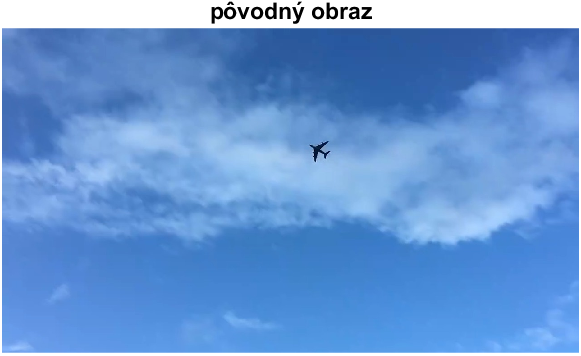
\includegraphics[width=.3\textwidth]{obrazky/threshold/img.png}};
            \node (image2) [right of=image1] {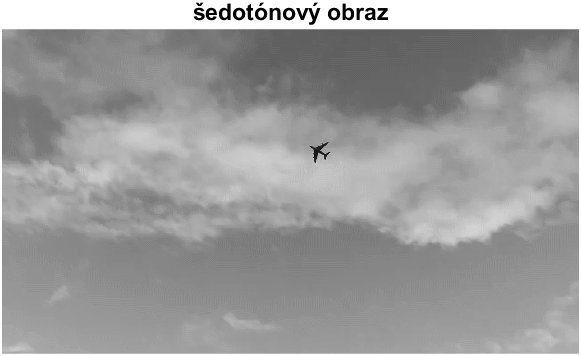
\includegraphics[width=.3\textwidth]{obrazky/threshold/img_gray.png}};
            \node (image3) [right of=image2] {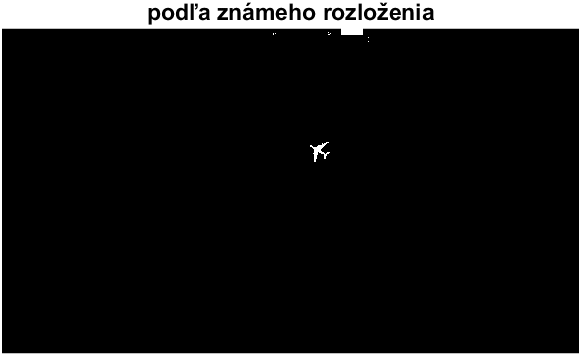
\includegraphics[width=.3\textwidth]{obrazky/threshold/img_thresh_distr.png}};

            \draw[->] (image1) -- (image2) node[midway, above] {};
            \draw[->] (image2) -- (image3) node[midway, above] {};
        \end{tikzpicture}
        \begin{tikzpicture}[>=stealth, node distance=5cm]
            \node (image1) {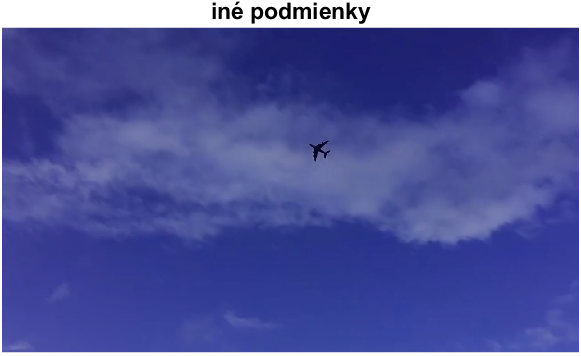
\includegraphics[width=.3\textwidth]{obrazky/threshold/img_dark.png}};
            \node (image2) [right of=image1] {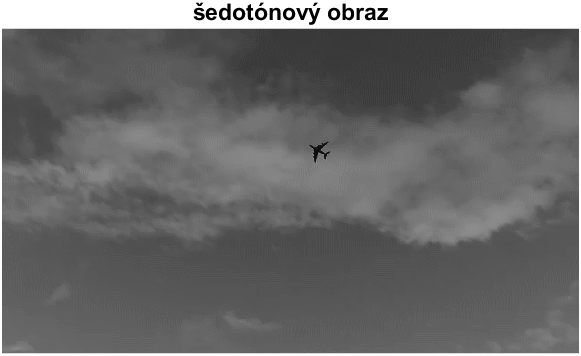
\includegraphics[width=.3\textwidth]{obrazky/threshold/img_dark_gray.png}};
            \node (image3) [right of=image2] {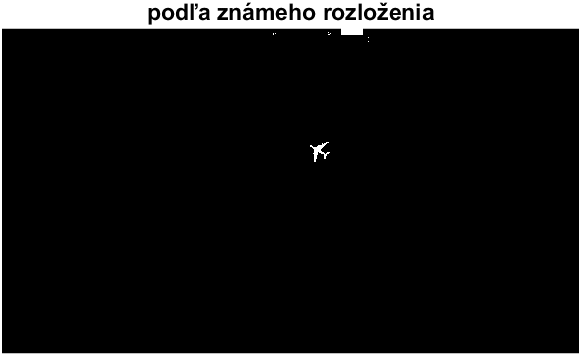
\includegraphics[width=.3\textwidth]{obrazky/threshold/img_thresh_distr.png}};

            \draw[->] (image1) -- (image2) node[midway, above] {};
            \draw[->] (image2) -- (image3) node[midway, above] {};
        \end{tikzpicture}
        \caption{Automatické prahovanie (podľa známeho rozloženia)}
    \end{figure}

\subsection{Lokálne prahovanie}

    V prípade že je jas pozadia rôzny v rôznych častiač obrazu, je vhodné určiť hodnotu prahu z jasovej úrovne okolia každého prahovaného pixelu. Toto takzvané adaptívne prahovanie, má síce vyžšiu výpočetnú náročnosť ako jednoduchšie globálne prahovanie, keďže je nutné určiť prah pre každý bod obrazu samostatne, je však robustnejšie voči nevhodnému pozadiu.

    \begin{figure}[!ht]
        \centering
        \begin{tikzpicture}[>=stealth, node distance=5cm]
            \node (image1) {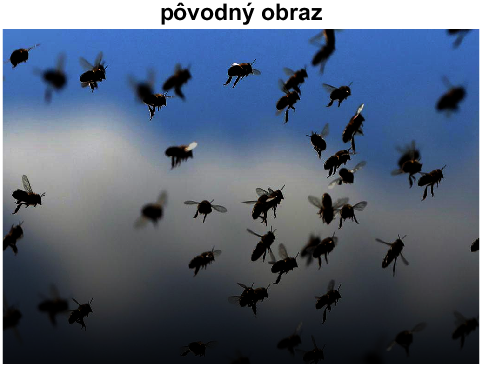
\includegraphics[width=.3\textwidth]{obrazky/threshold/img2.png}};
            \node (image2) [below of=image1] {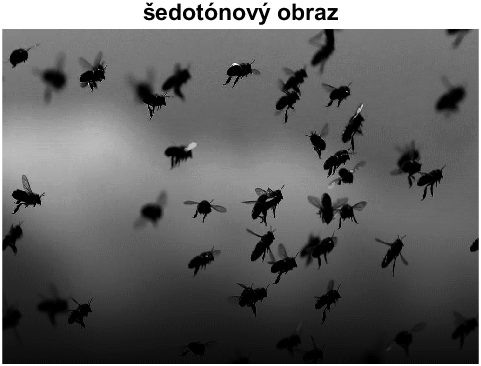
\includegraphics[width=.3\textwidth]{obrazky/threshold/img2_gray.png}};
            \node (image3) [left of=image2] {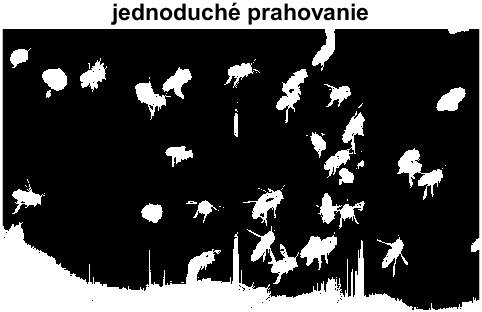
\includegraphics[width=.3\textwidth]{obrazky/threshold/img2_simple_thresh.png}};
            \node (image4) [right of=image2] {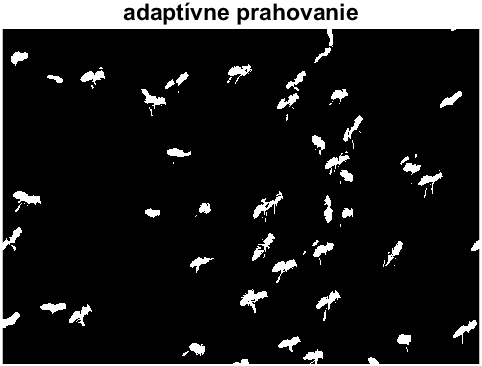
\includegraphics[width=.3\textwidth]{obrazky/threshold/img2_adaptive_thresh.png}};

            \draw[->] (image1) -- (image2) node[midway, above] {};
            \draw[->] (image2) -- (image3) node[midway, above] {};
            \draw[->] (image2) -- (image4) node[midway, above] {};
        \end{tikzpicture}
        \caption{Adaptívne prahovanie (podľa známeho rozloženia)}
    \end{figure}

\section{Detekcia hrán}

    Ako jednu z metód vyhľadávania objektov v obraze je možné využiť obraz hrán a vyhľadať v ňom kontúry objektov. Opäť existuje niekoľko spôsobov ako získať obraz hrán a ako ho využiť k segmentácii obrazu, teda k detekcii objektov.

    Na vytvorenie obrazu hrán z nasnímaného obrazu sa používa konvolúcia obrazu s operátorom navrhnutým tak aby aproximovalo deriváciu určitého rádu. Medzi často používané operátory patria Prewittov a Sobelov operátor, ktoré aproximujú prvú deriváciu v určitom smere (horizontálnom, vertikálnom, diagonálne). Druhú deriváciu aproximuje Laplaceov operátor, používa sa tiež v kombinácii s Gaussovým filtrom (LoG operátor), čo má za následok zníženie citlivosti na šum.

    % konvolučné operátory - hranové detektory
    \begin{figure}[!ht]
        \centering

        \begin{minipage}[b]{0.2\textwidth}
            \[
                \begin{bmatrix}
                    -1 & 0 & 1 \\
                    -1 & 0 & 1 \\
                    -1 & 0 & 1 \\
                \end{bmatrix}
            \]
            \centering
            Prewittov operátor
        \end{minipage}
        %
        \begin{minipage}[b]{0.2\textwidth}
            \[
                \begin{bmatrix}
                    -1 & 0 & 1 \\
                    -2 & 0 & 2 \\
                    -1 & 0 & 1 \\
                \end{bmatrix}
            \]
            \centering
            Sobelov operátor
        \end{minipage}
        %
        \begin{minipage}[b]{0.2\textwidth}
            \[
                \begin{bmatrix}
                    0 &  1 & 0 \\
                    1 & -4 & 1 \\
                    0 &  1 & 0 \\
                \end{bmatrix}
            \]
            \centering
            Laplaceov operátor
        \end{minipage}
        
        \begin{minipage}[b]{0.4\textwidth}
            \[
                \begin{bmatrix}
                    0 & 0 & -1 & 0 & 0 \\
                    0 & -1 & -2 & -1 & 0 \\
                    -1 & -2 & 16 & -2 & -1 \\
                    0 & -1 & -2 & -1 & 0 \\
                    0 & 0 & -1 & 0 & 0 \\
                \end{bmatrix}
            \]
            \centering
            LoG operátor
        \end{minipage}
    \end{figure}

    Komplexnejšiou metódou detekcie hrán je takzvaný \emph{Cannyho hranový detektor}. Ide o proces vo viacerých krokoch, pre jeden vstupný obraz sa postupuje nasledovne:

    \begin{enumerate}
        \item Vstupný obraz býva väčšinou filtrovaný z dôvodu zníženia citlivosti na šum v obraze. Vhodné je k tomu napríklad Gaussove rozmazanie.
        
        \item Použije sa horizontálny a vertikálny Sobelov operátor ako detektor hrán, na získanie obrazu hrán v oboch smeroch \(I_{x}\) a \(I_{y}\).

        \begin{minipage}[b]{0.4\textwidth}
            \[I_{x} = 
            \begin{bmatrix}
                -1 & 0 & 1 \\
                -2 & 0 & 2 \\
                -1 & 0 & 1 \\
            \end{bmatrix}
            \ast I
            \]
        \end{minipage}
        %
        \begin{minipage}[b]{0.4\textwidth}
            \[I_{y} = 
            \begin{bmatrix}
                 1 &  2 &  1 \\
                 0 &  0 &  0 \\
                -1 & -2 & -1 \\
            \end{bmatrix}
            \ast I
            \]
        \end{minipage}

        \item Z toho je možné určiť magnitúdu a smer gradientu:
        
        \begin{minipage}[b]{0.4\textwidth}
            \[G = \sqrt{I_x^2 + I_y^2}\]
        \end{minipage}
        \begin{minipage}[b]{0.4\textwidth}
            \[\theta = atan2(I_x, I_y)\]
        \end{minipage}
        
        \item Ku zníženiu redundancie detekovaných hrán sa použije algorytmus \emph{non maxima suppression} (potlačenie nemaximálnej hodnoty). Použitím tohoto algorytmu dôjde k zúženiu hrán, pričom sa ponechajú len tie časti hrán ktorých magnitúda je väčšia ako v ich okolí.
        
        \item Dvojitým prahovaním sa v obraze hrán nájdu tri úrovne:
            \begin{itemize}
                \item \textbf{silné hrany} sú hrany vyššie ako obidva prahy. Do výsledného obrazu hrán sú určite pridané.
                \item \textbf{slabé hrany} sú hrany medzi dvomi prahmi.
                \item \textbf{nie hrany} sú tie hrany ktorých magnitúda je nižšia ako obidva prahy.
            \end{itemize}
            
        \item Iteratívne sú slabé hrany dotýkajúce sa silných hrán označované za silné, až kým sa žiadna slabá hrana silnej nedotýka. Vo výslednom obraze sú ponechané len silné hrany.
    \end{enumerate}

    \begin{figure}[!ht]
        \centering
        \begin{tikzpicture}[>=stealth, node distance=5cm]
            \node (image1) {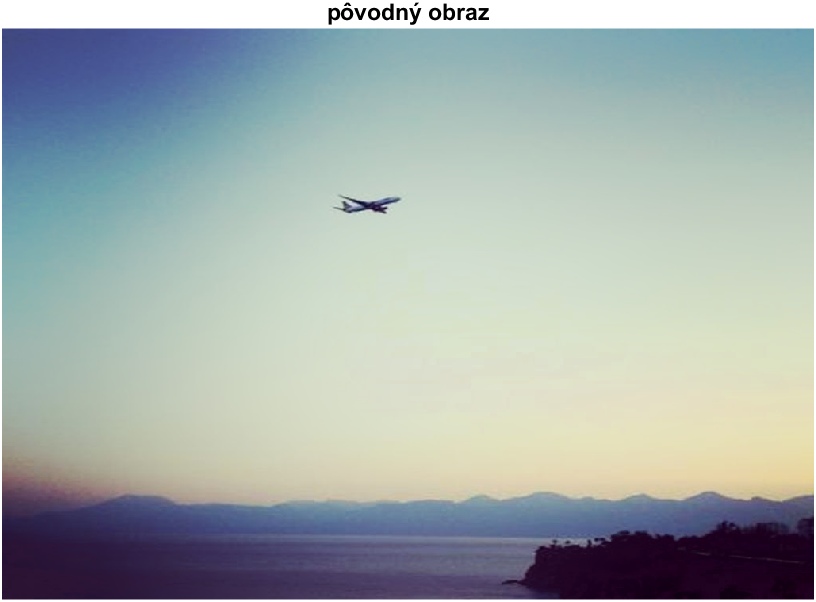
\includegraphics[width=.3\textwidth]{obrazky/canny/img.png}};
            \node (image2) [right of=image1] {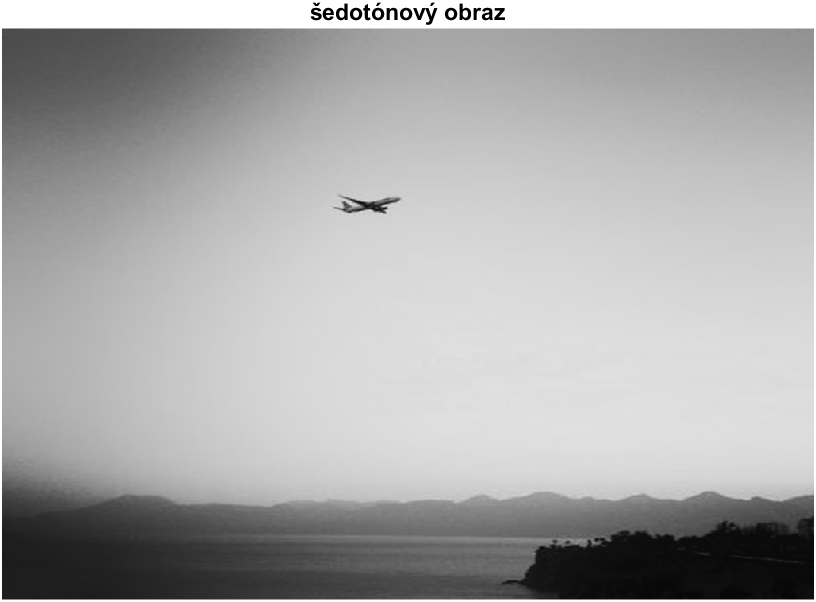
\includegraphics[width=.3\textwidth]{obrazky/canny/img_gray.png}};
            \node (image3) [right of=image2] {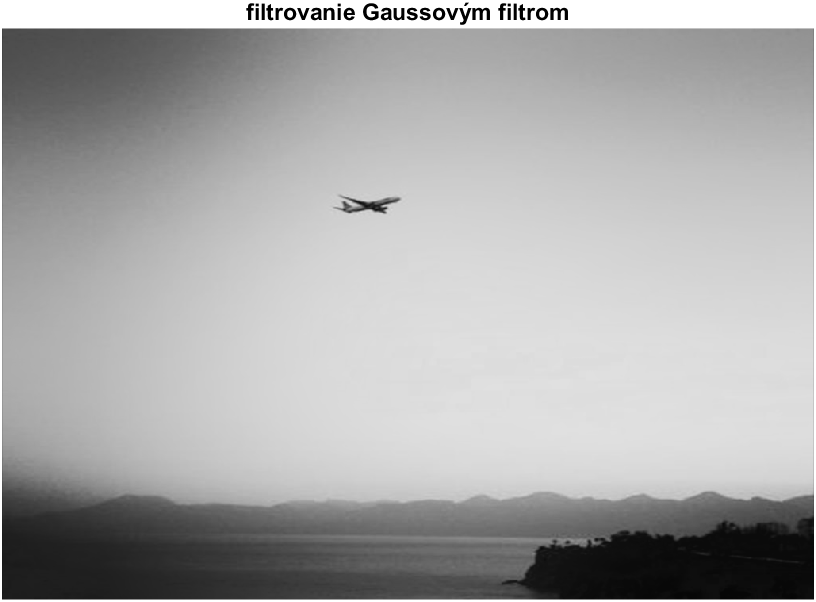
\includegraphics[width=.3\textwidth]{obrazky/canny/img_gauss.png}};
            \node (image4) [below of=image2] {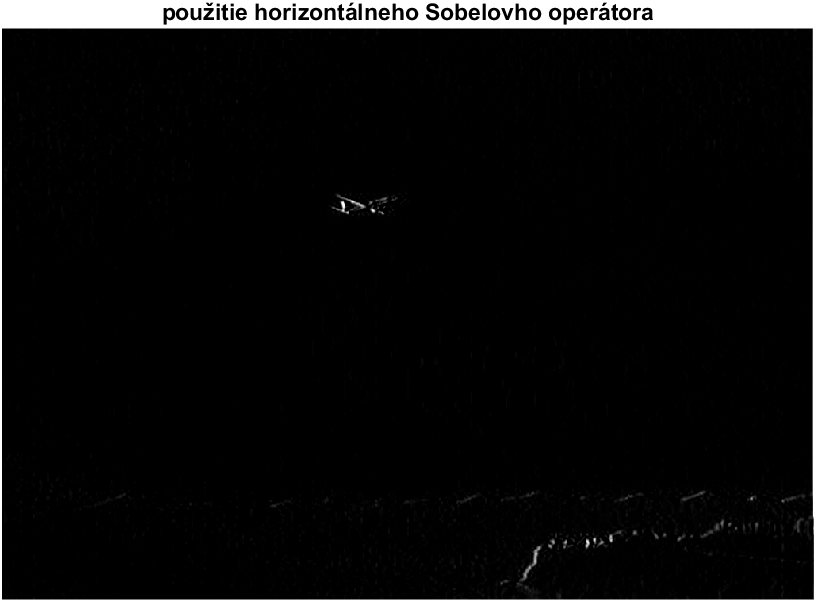
\includegraphics[width=.3\textwidth]{obrazky/canny/img_sobel_x.png}};
            \node (image5) [right of=image4] {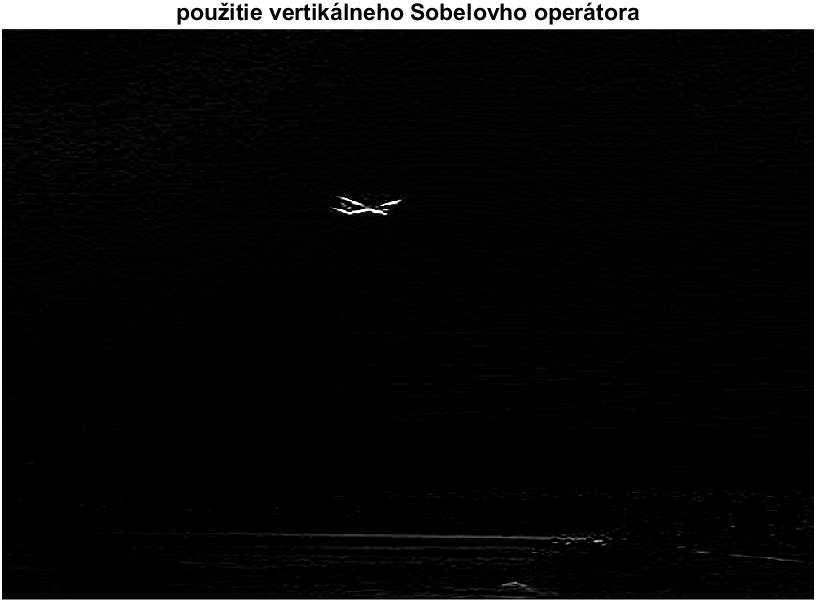
\includegraphics[width=.3\textwidth]{obrazky/canny/img_sobel_y.png}};
            \node (image6) [below of=image5] {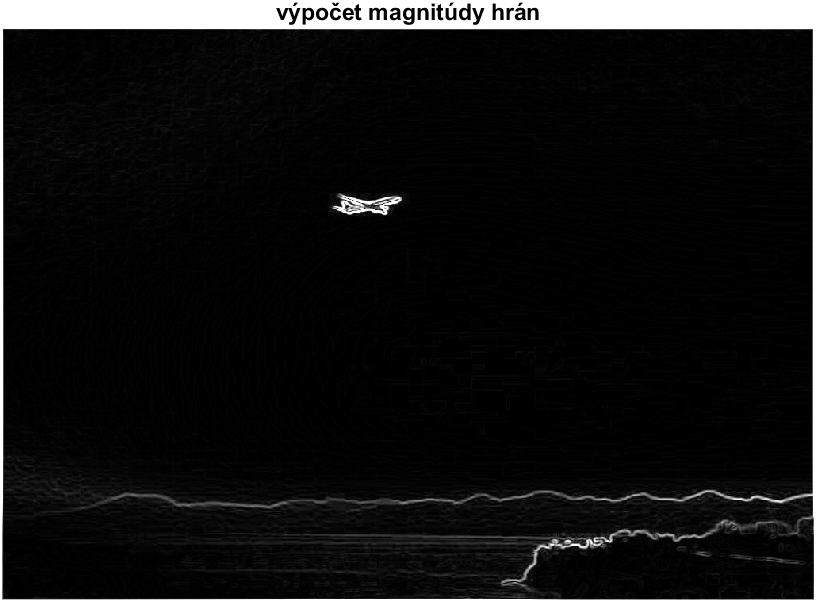
\includegraphics[width=.3\textwidth]{obrazky/canny/img_mag.png}};
            \node (image7) [left of=image6] {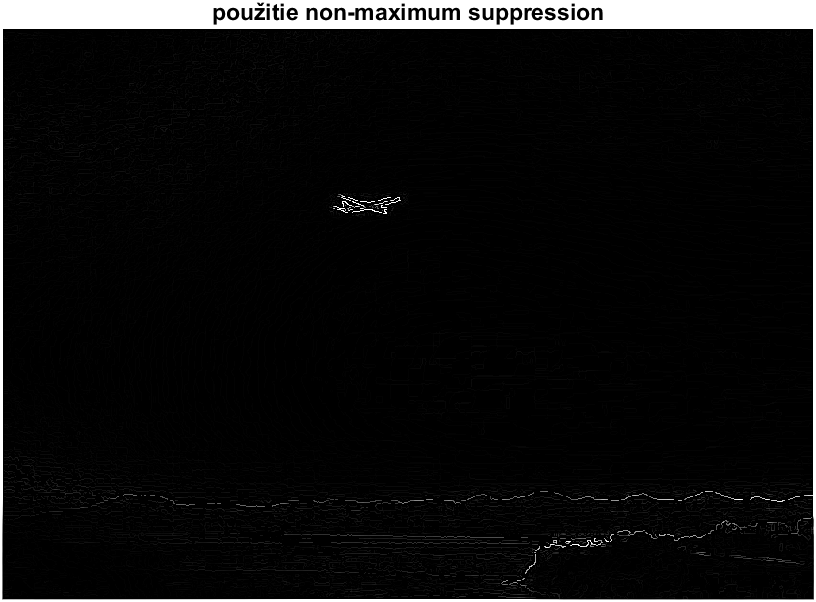
\includegraphics[width=.3\textwidth]{obrazky/canny/img_nms.png}};
            \node (image8) [left of=image7] {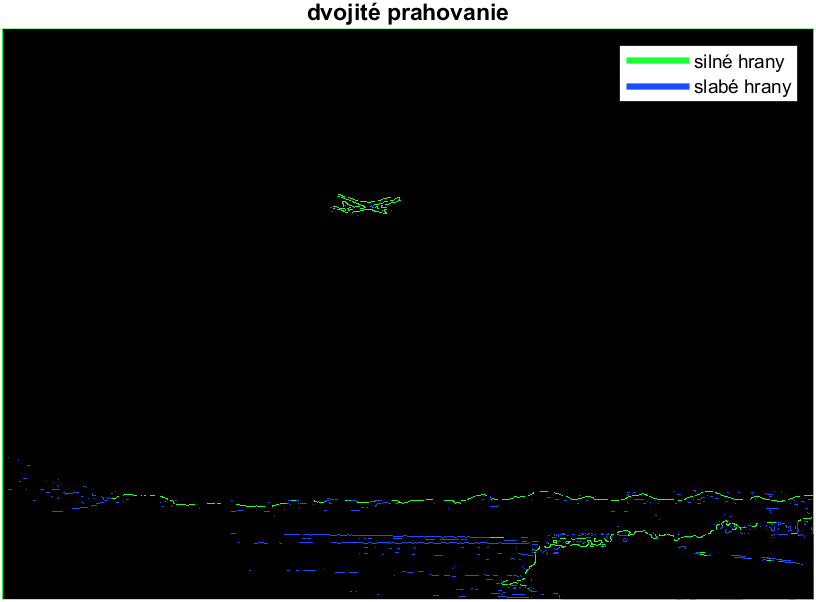
\includegraphics[width=.3\textwidth]{obrazky/canny/img_double_thresh.png}};
            \node (image9) [above of=image8] {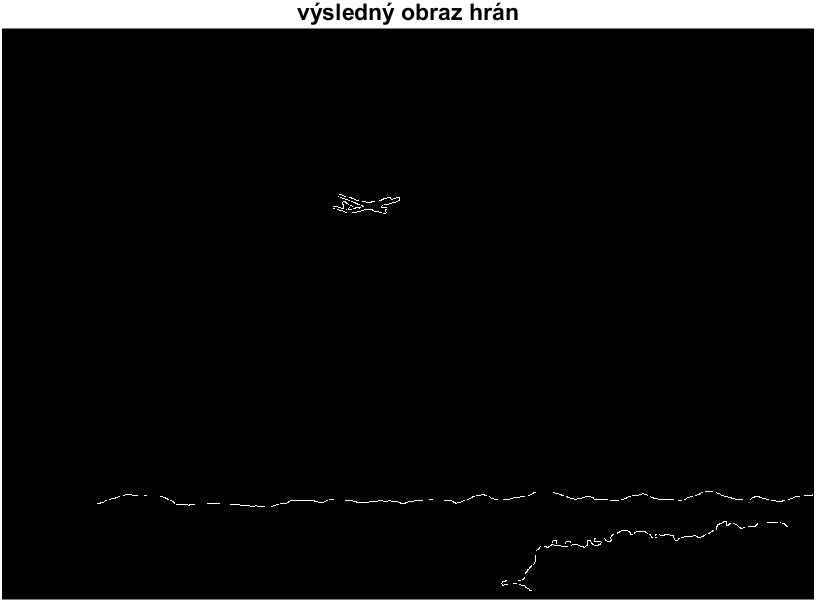
\includegraphics[width=.3\textwidth]{obrazky/canny/img_canny.png}};

            \draw[->] (image1) -- (image2) node[midway, above] {};
            \draw[->] (image2) -- (image3) node[midway, above] {};
            \draw[->] (image3) -- (image4) node[midway, above] {};
            \draw[->] (image3) -- (image5) node[midway, above] {};
            \draw[->] (image4) -- (image6) node[midway, above] {};
            \draw[->] (image5) -- (image6) node[midway, above] {};
            \draw[->] (image6) -- (image7) node[midway, above] {};
            \draw[->] (image7) -- (image8) node[midway, above] {};
            \draw[->] (image8) -- (image9) node[midway, above] {};
        \end{tikzpicture}
        \caption{Cannyho hranový detektor}
    \end{figure}

    Obraz hrán je možné ďalej spracovávať, napríklad morfologickýmy operáciami: otvorením odstrániť krátke nevýznamné hrany, zatvorením spojiť hrany blízko pri sebe.

    Vyhľadávaním uzavertých kontúr v obraze hrán je možné identifikovať potenciálne objekty v obraze.

    \subsection{Detekcia horizontu pomocou Houghovej transformácie}

        Pokiaľ časť obrazu obsahuje horizont, je vhodnejšie detekovať lietajúce objekty len na oblohe nad ním, aby sa predišlo falošným detekciám. Horizont je možné detekovať z obrazu hrán pomocou Houghovej transformácie, podľa práce. Vo výsledku Houghovej transformácie sa horizont prejaví ako najvýraznejšia čiara.


        \begin{figure}[H]
            \centering
            \begin{tikzpicture}[>=stealth, node distance=8cm]
                \node (image1) {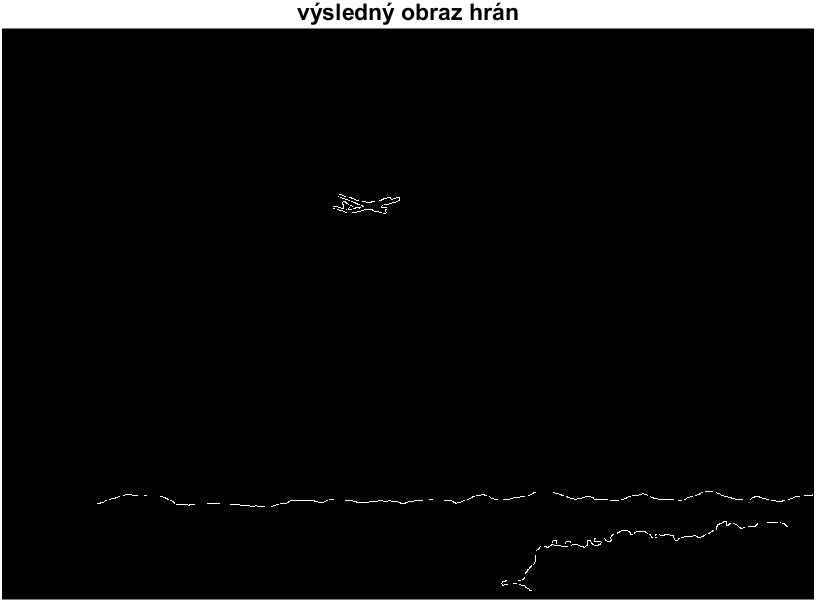
\includegraphics[width=.4\textwidth]{obrazky/canny/img_canny.png}};
                \node (image2) [below of=image1, yshift=2.5cm] {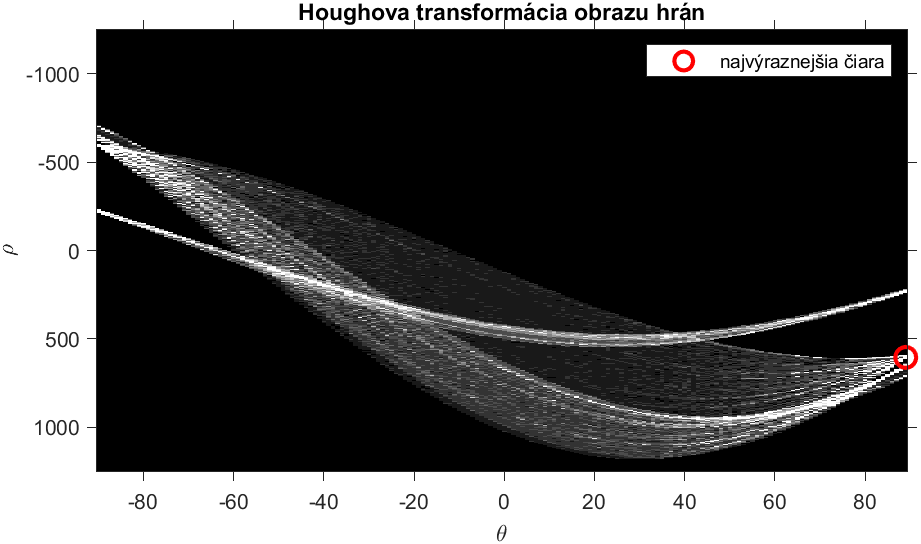
\includegraphics[width=.45\textwidth]{obrazky/canny/img_hough.png}};
                \node (image3) [right of=image2] {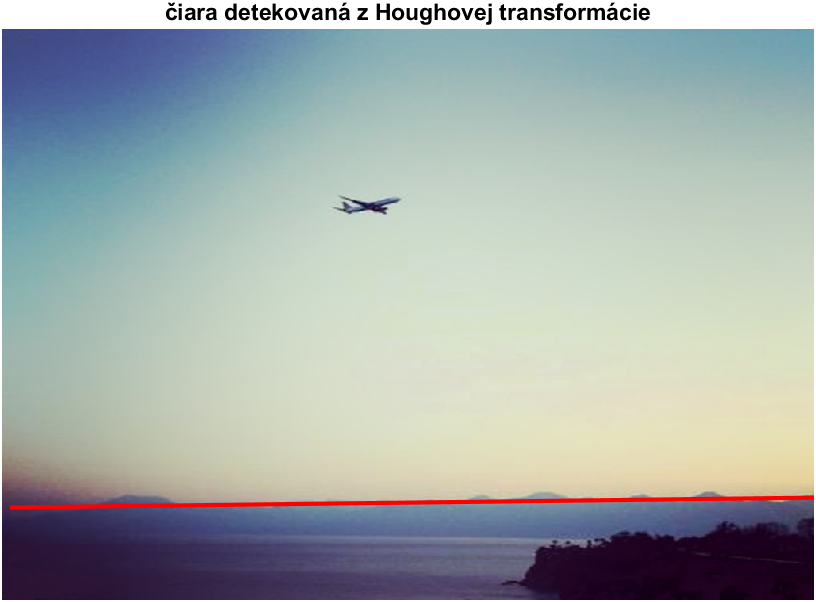
\includegraphics[width=.4\textwidth]{obrazky/canny/img_horizon.png}};

                \draw[->] (image1) -- (image2) node[midway, above] {};
                \draw[->] (image2) -- (image3) node[midway, above] {};
            \end{tikzpicture}
            \caption{Detekcia horizontu pomocou Houghovej transformácie}
        \end{figure}

\section{Detekcia pohybu}

    V prípade že je požadovaná detekcia pohybujúcich sa objektov, je možnosťou detekcie práve detekovaním ich pohybu. Jednou z jednoduchých metód detekcie pohybu sú rozdielové metódy, pri ktorých je vypočítavaný rozdielový snimok z viacerých snímkov zo sekvencie \(\{I_1, I_2, ..., I_n\}\). Rozdielový snímok môže byť:

    \begin{itemize}
        \item \textbf{jednostranný} - je najjednoduchší nenesie informáciu o smere pohybu, vyhodnocuje sa len v miestach kde \(I_1(x,y) > I_2(x,y)\).
        \[D(x,y) = \begin{cases}
            0 & I_1(x,y) - I_2(x,y) < \epsilon \\
            1 & I_1(x,y) - I_2(x,y) \geq \epsilon
        \end{cases}\]

        \item \textbf{obojstranný} - dostaneme ho upravením vzťahu pre jednostranný rozdielový snímok, použitím absolútnej hodnoty. Tým je dosiahnutá zameniteľnosť \(I_1(x,y)\) a \(I_2(x,y)\), vyhodnocuje sa teda na celom obraze. Neodstraňuje nedostatok informácie o smere pohybu, tá však nemusí byť nutnosťou.
        \[D(x,y) = \begin{cases}
            0 & |I_1(x,y) - I_2(x,y)| < \epsilon \\
            1 & |I_1(x,y) - I_2(x,y)| \geq \epsilon
        \end{cases}\]

        \item \textbf{kumulovaný} - je vytvorený váženým súčtom jedno alebo obojstranných rozdielových snímkov. Je teda možné priemerovať pohyb za určitý čas určením každej váhy \(\omega = 1/(N-1)\), alebo určiť rôznym snímkom rôznu váhu a získať tak informáciu o smere pohybu.
        \[D(x,y) = \sum_{i=1}^{N-1}\omega_i \cdot D_i(x,y)\]
    \end{itemize}

    Komplexnejšiou metódou detekcie pohybu je vytvorenie rozdielového snímku nie medzi nasledujúcimi snímkami, ale aktuálnym snímkom a vytvoreným modelom pozadia. Ten je možné zostaviť:

    \begin{itemize}
        \item ako jeden obraz pozadia bez objektov.
        \item ako priemerný snímok niekoľkých snímkov pozadia.
        \item ako dynamický model - iteratívnym aktualizovaním podľa aktuálneho snímku. Tým sa model pozadia postupne prispôsobuje malým zmenám v prostredí.
    \end{itemize}

    \begin{figure}[H]
        \centering
        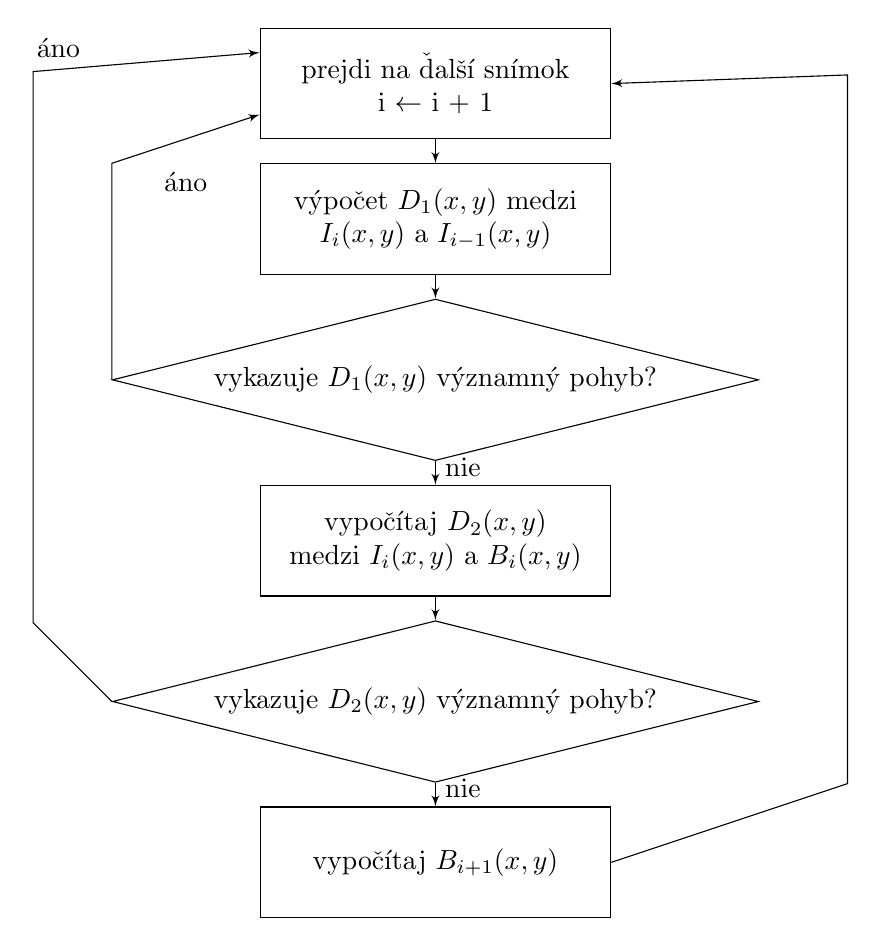
\begin{tikzpicture}[node distance=.3cm, auto]

            % Define block styles
            \tikzstyle{block} = [rectangle, draw, fill=white!20, text width=12em, text centered, sharp corners, minimum height=4em]
            \tikzstyle{line} = [draw, -latex']

            % Nodes
            \node [block] (start) {prejdi na ďalší snímok
            
            i \(\leftarrow\) i + 1};
            \node [block, below=of start] (calc_d1) {výpočet \(D_1(x,y)\) medzi \(I_i(x,y)\) a \(I_{i-1}(x,y)\)};
            \node [draw, diamond, aspect=4, below=of calc_d1] (check_d1) {vykazuje \(D_1(x,y)\) významný pohyb?};
            \node [block, below=of check_d1] (calc_d2) {vypočítaj \(D_2(x,y)\) medzi \(I_i(x,y)\) a \(B_i(x,y)\)};
            \node [draw, diamond, aspect=4, below=of calc_d2] (check_d2) {vykazuje \(D_2(x,y)\) významný pohyb?};
            \node [block, below=of check_d2] (calc_b) {vypočítaj \(B_{i+1}(x,y)\)};

            % Arrows
            \path [line] (start) -- (calc_d1);
            \path [line] (calc_d1) -- (check_d1);
            \path [line] (check_d1.west) -- ++(0,2.75) -- node [below = .3cm] {áno} (start.190);
            \path [line] (check_d1) -- node [near start] {nie} (calc_d2);
            \path [line] (calc_d2) -- (check_d2);
            \path [line] (check_d2.west) -- ++(-1,1) -- ++(0,7) -- node [near start] {áno} (start.170);
            \path [line] (check_d2) -- node [near start] {nie} (calc_b);
            \path [line] (calc_b.east) -- ++(3,1) -- ++(0,9) -- (start.east);

        \end{tikzpicture}
        \caption{Postup aktualizovania dynamického modelu pozadia}
    \end{figure}

    Výpočet nového modelu pozadia \(B_{i+1}(x,y)\) môže prebiehať napríklad pomocou lineárneho zabúdania, teda \(B_{i+1}(x,y) = \alpha \cdot I_i(x,y) + (1 - \alpha) \cdot B_i(x,y)\).

    Obraz obsahujúci detekovaný pohyb je získaný rozdielom a prahovaním aktuálneho snímku a modelu pozadia.

    \begin{figure}[H]
        \centering
        \begin{tikzpicture} [node distance=1.5cm, auto]
            \node (image1) {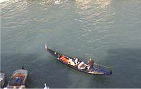
\includegraphics[width=.3\textwidth]{obrazky/motion/frame.png}};
            \node (space1) [below of=image1] {};
            \node (image2) [below of=space1] {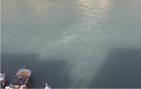
\includegraphics[width=.3\textwidth]{obrazky/motion/background.png}};
            \node (sum) [draw, rectangle, right of=space1, xshift=2.5cm] {D(x,y)};
            \node (threshold) [draw, rectangle, right of=sum, xshift=.5cm] {\(\geq \epsilon\)};
            \node (image3) [right of=threshold, xshift=2.5cm] {
\includegraphics[width=.3\textwidth]{obrazky/motion/motion.png}};

            \draw[->] (image1.east) to [out=0, in=90] (sum.north);
            \draw[->] (image2.east) to [out=0, in=270] (sum.south);
            \draw[->] (sum) -- (threshold);
            \draw[->] (threshold) -- (image3);
        \end{tikzpicture}
        \caption{Odčítanie pozadia}
    \end{figure}

\chapter{Popis objektov}

    \section{príznaky}

\chapter{Klasifikácia}

    Ďalším krokom je určenie triedy detekovaných objektov, teda ich klasifikácia. Tá môže byť vykonaná na základe obrazu, alebo pomocou príznakov získaných z neho.

    \section{Konvolučné neurónové siete}

        Na rozdiel od plne prepojenej neurónovej siete, sú \ac{CNN} prispôsobené na prácu s obrazom ako so vstupným signálom. Ich architektúra je usporiadaná do vrstiev, štandardne po sebe nasledujú:

        \begin{enumerate}
            \item \textbf{Konvolučná vrstva} - používa konvolučné filtre na extrakciu príznakov z obrazu.
            \item \textbf{Aktivačná vrstva} - aplikuje aktivačnú funkciu, často napríklad \ac{ReLU} na každý bod. Zavádza do siete nelinearitu a pomáha zachytávať zložitejšie vzory.
            \item \textbf{Pooling vrstva} - redukuje priestorové rozlíšenie vstupných dát. Tým sa zníži výpočtová náročnosť nasledujúcich vrstiev. Najčastejšie sa používa \emph{max pooling}, teda výber najvyššej hodnoty v okolí.
        \end{enumerate}

        Väčšinou je použitá kombinácia niekoľko \textbf{konvolučných} vrstiev nasledovaných \textbf{aktivačnou} vrstvou, po ktorých \textbf{pooling} vrstva pripraví redukovaný vstup pre ďalšie vrstvy. Takýchto kombinácii nasleduje niekoľko, posledná je pripojená na plne prepojenú neurónovú sieť. Konvolučná časť slúži na vyhľadávanie príznakov, plne prepojená časť na klasifikáciu pomocou nich.

        \begin{figure}[h]
            \centering
            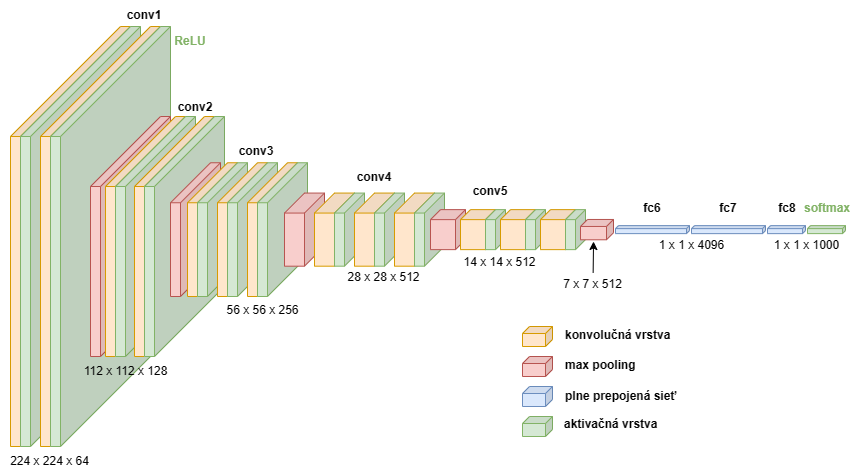
\includegraphics[width=.9\textwidth]{obrazky/cnn/cnn.png}
            \caption{Príklad architektúry konvolučnej neurónovej siete}
        \end{figure}

        Rozmery vrstiev závisia na tvare vstupného signálu. V prípade šedotónového obrazu je každý bod obrazu reprezentovaný jednou skalárnou hodnotou, v prípade farebného záleží počet hodnôt na pixel na farebnom modele. Klasifikáciou z farebného obrazu získavame väčšie množstvo informácii ale je vyžadovaný vyšší výkon, nakoľko sa konvolučné filtre aplikujú po jednom na každú zložku obrazu (teda v prípade RGB modelu na červenú, zelenú a modrú zložku samostatne).

        Výstup z poslednej vrstvy plne prepojenej časti siete je výstupom z celej \ac{CNN}. Výstupy klasifikačnej neurónovej siete s úlohov klasifikovať viacero tried, mávajú formáty:

        \begin{itemize}
            \item Jeden výstup, ktorého hodnota určuje triedu do ktorej sú vstupné dáta sieťou priradené.
            \item Vektor výstupov výstupov s toľkými hodnotami, na koľko tried je naučená sieť klasifikovať. Hodnoty výstupov môžu reprezentovať:
            \begin{itemize}
                \item Ohodnotenie triedy (score-based classification). V tomto prípade čísla na výstupe nemajú samostatne význam, ale ako predpoveď je určená trieda s najvyšším skóre.
                \item Pravdepodobnosť zaradenia do danej triedy. Tá je získaná použitím výstupnej aktivačnej vrstvy typu \emph{softmax}, ktorá spôsobí že každý z výstupov má hodnotu od 0 do 1 a súčet všetkých výstupov je 1.
            \end{itemize}
        \end{itemize}
        

\chapter{Detekcia a klasifikácia v jednom kroku}

    \section{R-CNN}

        \ac{R-CNN} sú skupina modelov strojového učenia zaločená na \ac{CNN}. Ich cieľom je nájdenie a klasifikovanie objektov v obraze. Ich výstupom je množina rámčekov ohraničujúcich objekty a im pridelené triedy.

        \ac{R-CNN} pracujú v niekoľkých etapách:
        \begin{enumerate}
            \item \textbf{Selektívne vyhľadávanie} - vstupný obraz je spracovaný a sú extrahované \ac{RoI}, teda orámované oblasti obrazu, ktoré by mohli obsahovať objekty alebo ich časti. Počet takto navrhovaných oblastí môže dosahovať niekoľko tisíc.
            \item \textbf{Extrakcia príznakov} - každý \ac{RoI} je predložený ako vstup pre naučenú \ac{CNN}, ktorá vyprodukuje príznakový vektor pre každý \ac{RoI}.
            \item \textbf{Klasifikácia} - pomocou skupiny modelov \ac{SVM} je podľa príznakov extrahovaných \ac{CNN}, klasifikovaný každý \ac{RoI} do jednej z určených tried alebo ako pozadie - teda nepatriaci do žiadnej triedy.
            \item \textbf{Regresia ohraničení} - konečný krok, zvyšujúci presnosť orámovania objektov. Používa sa pri ňom naučený model nezávyslý na mierka nazývaný \emph{bounding box regressor}. Jeho výstup je štvorrozmerný, skladá sa z polohy a rozmerov ohraničujúceho obdĺžnika.
        \end{enumerate}

        \ac{R-CNN} sú efektívne, no náročné na výpočetný výkon. Z toho dôvodu boli vyvinuté rýchlejšie varianty \emph{Fast R-CNN} a \emph{Faster R-CNN}.

        \emph{Fast R-CNN} aplikuje \ac{CNN} na celý vstupný obraz a extrahuje z neho mapu príznakov. Až na výslednú mapu aplikuje takzvaný \ac{RoI} \emph{pooling}, ktorý extrahuje príznaky pre každý \ac{RoI}, pomocou okna pevnej veľkosti. Zvyšok modelu pracuje podobne ako \ac{R-CNN}, s využitím plne prepojenej siete na klasifikáciu a generovanie orámovaní.

        \emph{Faster R-CNN} nadväzuje na \emph{Fast R-CNN} nahradením selektívneho vyhľadávania modelom typu \ac{RPN}. Vstupný obraz prechádza predučenou \ac{CNN}, sú extrahované príznaky. \ac{RPN} využije nájdené príznaky aby určila kde sa nachádzajú potenciálne objekty v obraze. V konečnom kroku sú klasifikované navrhnuté ohraničené oblasti podľa príznakov extrahovaných v predošlom kroku. \emph{Faster R-CNN} je dostatočne rýchla na použitie v reálnom čase.

    \section{YOLO}

        \ac{YOLO} je populárny algorytmus detekcie, ktorý na rozdiel od \ac{R-CNN} rozdeľuje obraz do mriežky a postupne aplikuje klasifikátor. Postupuje nasledovne:

        \begin{enumerate}
            \item Vstuný obraz je rozdelený na mriežku \(S \times S\), ktorej veľkosť závisí na verzii \ac{YOLO}.
            \item V každej bunke mriežky je predikovaný určitý počet ohraničených oblastí a im priradené skóre dôveryhodnosti. Tie značia úroveň istoty že oblasť obsahuje objekt a že dané ohraničenie je správne.
            \item Je použitých viacero klasifikátorov. \ac{YOLO} predikuje viacero oblastí za každú bunku. Počas trénovania je jednému z prediktorov udelená zodpovednosť za predikovanie daného objekto podľa toho ktorý z nich dosahuje najväčší \ac{IOU}.
            \item Každá bunka predikuje rozdelenie pravdepodobnosti všetkých tried.
        \end{enumerate}

        Hlavnou výhodou \ac{YOLO} je rýchlosť. Všeobecne pracuje rýchlejšie a s menším požadovaným výpočetným výkonom. Na druhú stranu má nevýhody spôsobené obmedzením veľkosti orámovaných oblastí. Presnosť \ac{YOLO} býva nižšia pri primalých objektoch, pre použitia vyžadujúce vyžšiu presnosť sa môže javiť ako výhodnejšie použiť iné modely.

\chapter{Návrh kombinácie a usporiadania hardvérových komponentov}

    Táto kapitola sa zameriava na návrh a implementáciu prenosného zariadenia pre detekciu, klasifikáciu a trasovanie lietajúcich objektov. Cieľom návrhu je vytvorenie zariadenia s možnosťou nasadenia v čo najrôznejších podmienkach. Jednou z podminok je teda jeho prenosnosť, možnosť napájania z akumulátoru a nezávyslosť na iných zariadeniach pri jeho nastavení a používaní.

    \section{Jednodoskový počítač}
    
        Jedným z najčastejšie používaných jednodoskových počítačov je rada \emph{Raspberry Pi}. V čase návrhu bol najnovším model \emph{Pi 4 model B}. Tento model disponuje:
        \begin{itemize}
            \item 1.5GHz ARM Cortex-A72 procesorom so 4 jadrami,
            \item do 8 Gb pamäte RAM,
            \item rozhraním HDMI s možnosťou pripojenia dvoch monitorov,
            \item 4 USB, z toho 2 USB 3.0,
            \item MIPI CSI konektor pre pripojenie kamery.
        \end{itemize}

        Ďalšou možnosťou je použitie jednodoskového počítača špeciálne navrhnutého na použitie v aplikáciách počítačového videnia, či všeobecne umelej inteligencie (Nvidia Jetson Xavier, Google Coral Dev Board, Rock Pi, Nvidia Jetson Nano, a podobné). \emph{Raspberry Pi} má v porovnaní nižší odber, je kompaktnejšie, jednoduché na použitie a má dobrú kompatibilitu s operačnými systémamy. Dokumentácia a knižnice pre \emph{Raspberry Pi} sú jednoducho dostupné a zariadenia majú garantovanú dlhodobú podporu software aj hardware.

        Z týchto dôvodov bolo \emph{Raspberry Pi} zvolené na použitie v zariadení.

    \section{Kamera}

        \emph{Raspberry Pi} dovoľuje pripojenie kamery cez MIPI konektor. Je teda najjednoduchšie použiť kamerový modul vyrobený konkrétne pre \emph{Raspberry Pi}. Najaktuálnejší oficiálny \emph{Raspberry Pi} kamerový modul v čase návrhu je 12Mpx \emph{Raspberry Pi Camera 3} so senzorom Sony IMX708 a automatickým ostrením. Parametre kamery a objektívu sú:
        \begin{itemize}
            \item \textbf{Ohnisková vzdialenosť:} 4,74 mm
            \item \textbf{Horizontálne zorné pole} 66 \(^\circ\)
            \item \textbf{Vertikálne zorné pole} 41 \(^\circ\)
        \end{itemize}

    \section{Ovládacie prvky}

        Ako najlepší ovládací a zobrazovací prvok bol z hľadiska prenosnosti a kompaktnosti zvolený dotykový displej, konkrétne 7 palcový IPS displej od firmy Waveshare. Táto veľkosť je postačujúca na zobrazovanie výsledkov detekcie aj ovládanie zariadenia. Rozhranie HDMI značne zjednodušuje prepojenie a inštaláciu displeja.

    \section{Uchytenie kamery}

        Praktickou výhodou prenosného zariadenia by bola možnosť jeho umiestnenia o statív. Keďže je cieľom kamerou mieriť smerom nahor, na oblohu, bolo by užívateľské rozhranie pri nesprávnej vzájomnej orientácii kamery a displeja natočené neprakticky nadol. Namiesto pevnej konfigurácie uhla medzi displejom a kamerou bolo navrhnuté pohyblivé uchytenie kamery v kryte zariadenia, vyrobiteľné 3D tlačou.

        \begin{figure}[H]
            \centering
            \begin{tikzpicture} [node distance=7cm, auto]
                \node (image1) {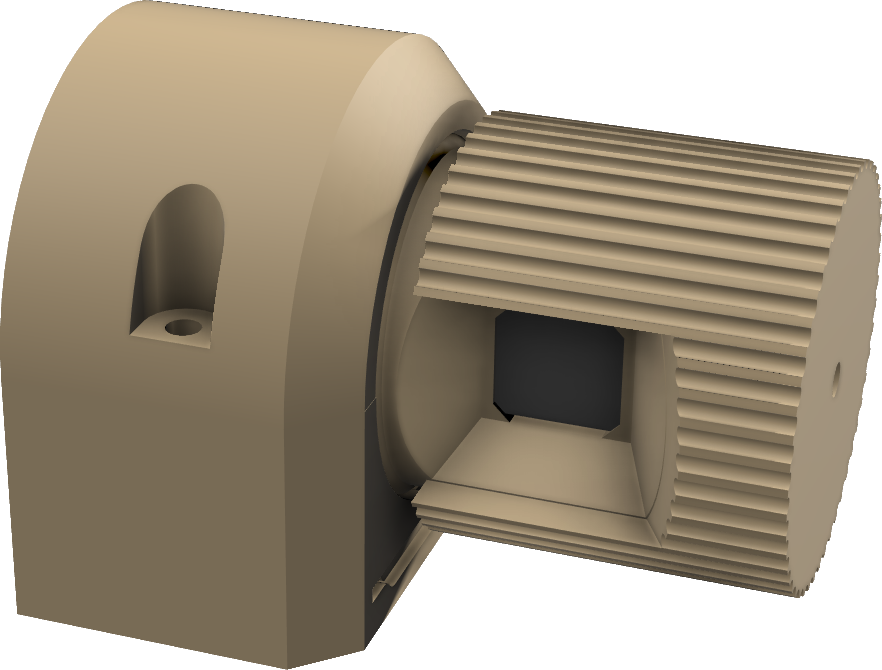
\includegraphics[width=.18\textwidth]{obrazky/case/camera_1.png}};
                \node (image2) [right of=image1] {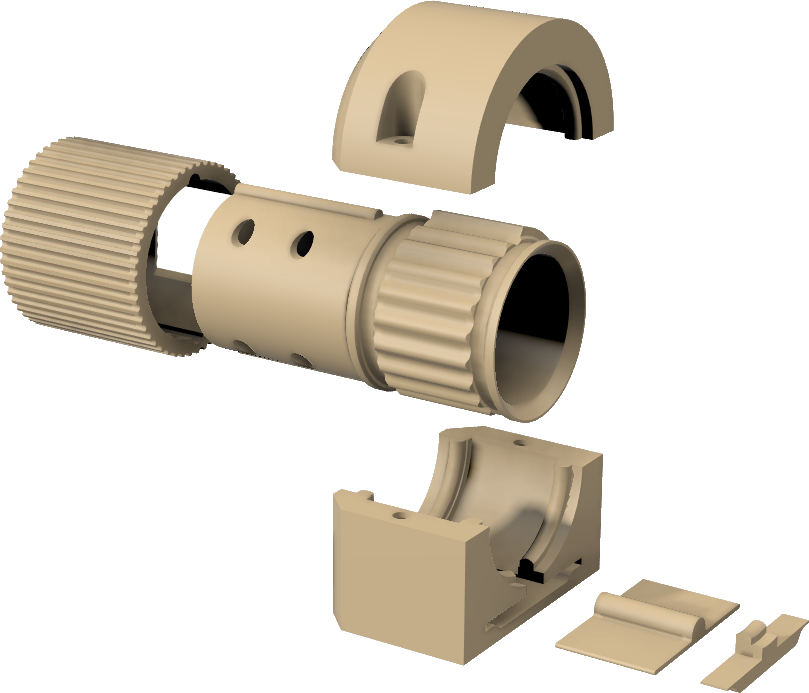
\includegraphics[width=.45\textwidth]{obrazky/case/camera_2.png}};
            \end{tikzpicture}
            \caption{návrh nastaviteľného uchytenia kamery}
        \end{figure}

        \begin{figure}[h]
            \centering
            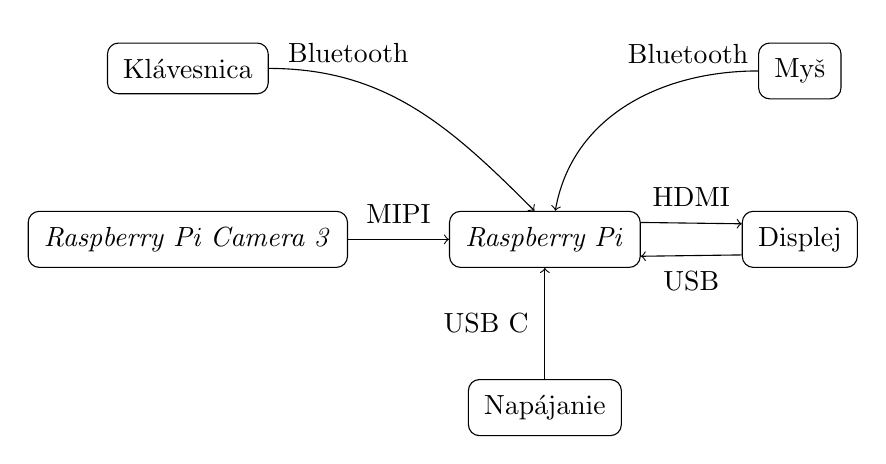
\begin{tikzpicture} [node distance=2.5cm, auto, inner sep=.2cm, rounded corners]
                \node (Pi) [draw, rectangle] at(0,0) {\emph{Raspberry Pi}};
                \node (Display) [right of=Pi, draw, rectangle, anchor=west] {Displej};
                \node (Camera) [left of=Pi, draw, rectangle, anchor=east] {\emph{Raspberry Pi Camera 3}};
                \node (Power) [below of=Pi, draw, rectangle, anchor=south] {Napájanie};
                \node (Keyboard) [above of=Camera, draw, rectangle, anchor=north] {Klávesnica};
                \node (Mouse) [above of=Display, draw, rectangle, anchor=north] {Myš};

                \draw[->] (Pi.10) -- (Display.165) node[midway, above] {HDMI};
                \draw[->] (Display.195) -- (Pi.350) node[midway, below] {USB};
                \draw[->] (Camera) -- (Pi) node[midway, above] {MIPI};
                \draw[->] (Power) -- (Pi) node[midway, left] {USB C};
                \draw[->] (Keyboard.east) to [out=. in=100] node[near start, above]{Bluetooth} (Pi.110);
                \draw[->] (Mouse.west) to [out=180, in=80] node[near start, above]{Bluetooth} (Pi.70);
            \end{tikzpicture}
            \caption{bloková schéma zariadenia}
        \end{figure}

\chapter{Tvorba datasetu}

    Správne naučenie modelov a ich schopnosť generalizovať z veľkej miery záleží na kvalite použitého datasetu (množiny dát). Tvorba datasetu je teda kľúčový krok pri práci so systémami strojového videnia.

    Cieľom pri tvorbe datasetu je zabezpečiť dostatočnú kvalitu a správnosť dát, dosiahnuť početne podobné zastúpenie každej triedy a správne reprezentovať rôznorodosť dát v rámci jednotlivých tried. Je vhodné aby boli vzorky získané pri rôznych podmienkach, podľa plánovaného použitia výsledného modelu.

    \section{Získavanie dát}

        Keďže táto práca nadväzuje na prácu \cite{Jurecka2021}, tvorí dataset v nej vytvorený základ pre ten použitý v tejto práci. Navyše bol rozšírený o niekoľko ďalších open source datasetov a vlastných anotovaných fotografii.

        Na tvorbu datasetu bol použitý program \emph{roboflow}, ktorý umožňuje načítavanie existujúcich datasetov, nahrávanie vlastných fotografii, anotáciu, spájanie dostupných datasetov, augmentácia datasetu a generovanie anotačných súborov rôznych formátov.

        Po pridaní všetkých častí datasetu a kontrole správnosti anotácie, boli počty inštancií jednotlivých tried:

        \begin{itemize}
            \item \textbf{vták}: 9047
            \item \textbf{dron}: 1190
            \item \textbf{helikoptéra}: 509
            \item \textbf{hmyz}: 249
            \item \textbf{lietadlo}: 845
        \end{itemize}

    \section{Úprava, rozdelenie a rozšírenie datasetu}

        Niektoré triedy sú reprezentované výrazne menším množstvom jednotlivých inštancii, čo je spôsobené nižšou dostupnosťou dát. Väčšina fotografii vtákov z vzdialenosti pri ktorej by mali byť detekované pochopiteľne obsahuje niekoľko desiatok jedincov, trieda vták je teda nadmerne zastúpená. Je možné tento problém čiastočne vyriešiť augmentáciou datasetu, čo program \emph{roboflow} umožňuje priamo pri generovaní novej verzie. V budúcnosti je vhodnejším riešením ďalšie rozšírenie datasetu o snímky s objektami aktuálne nedostatočne reprezentovaných tried.

        Aby bolo zabránené preučeniu modelu, musia byť dáta na ktorých je model učený rôzne od vylidačných a testovacích. Anotované obrazové dáta boli rozdelené do skupín s počtom:

        \begin{itemize}
            \item \textbf{trénovanie}: 2367
            \item \textbf{validácia}: 572
            \item \textbf{testovanie}: 290
        \end{itemize}

        Snímky boli predspracované upravením veľkosti na \(640 \times 640\) px a boli aplikované augmentácie, ktorými bol počet inštancií v trénovacej množine rozšírený na 7101:

        \begin{itemize}
            \item Rotácia \(-30^\circ\) až \(+30^\circ\)
            \item Zkosenie \(\pm 15^\circ\) vertikálne aj horizontálne
            \item Posun odtieňu \(-35^\circ\) až \(+35^\circ\)
            \item Zmena saturácie -25 \% až +25 \%
            \item Zmena expozície -20 \% až +20 \%
            \item Rozmazanie do 0,8 px
        \end{itemize}

    \section{Testovanie použiteľnosti datasetu}

    Použiteľnosť modelu bola testovaná naučením modelu typu \emph{Roboflow 3.0 Object Detection} priamo v aplikácii \emph{roboflow}, ktorý dosahoval úroveň presnosti 86.1 \% pri zvolenej variante modelu \emph{fast}. Pri dlhšom učení modelu určeného na reálne použitie sa dá predpokladať že dosiahnutá presnosť bude vyššia.

    Obrázok \ref{fig:roboflow_metrics} zobrazuje metriky presnosti naučeného modelu vypočítané v programe \emph{roboflow}, tak ako sa v ňom zobrazujú. Vypočítané metriky sú:

    \begin{itemize}
        \item \textbf{\ac{mAP}} \\ priemer priemerných presností za všetky triedy
        \item \textbf{Presnosť (Precision)} = \(\frac{TP}{TP + FP}\), značí s akou mieru správnej predikcie, v momente keď model nejakú hodnotu predikuje.
        \item \textbf{Senzitivita (Recall)} = \(\frac{TP}{TP + FN}\), na druhú stranu predstavuje pomer počtu správnych predikcii, ku počtu skutočne správnych hodnôt danej triedy.
    \end{itemize}

    \begin{figure}[H]
        \centering
        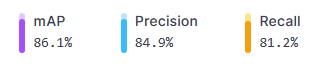
\includegraphics[width=.35\textwidth]{obrazky/roboflow/metrics.png}
        \caption{Metriky presnosti naučeného modelu v programe roboflow}
        \label{fig:roboflow_metrics}
    \end{figure}

    \begin{figure}[H]
        \centering
        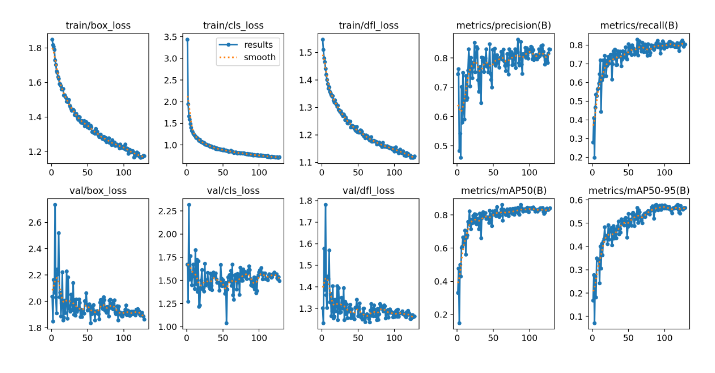
\includegraphics[width=.8\textwidth]{obrazky/roboflow/train.png}
        \caption{Grafické zobrazenie priebehu učenia modelu roboflow}
    \end{figure}

    Výsledná vygenerovaná verzia datasetu je z programu exportovateľná v niekoľkých formátoch, napríklad pre učenie siete \ac{YOLO} alebo pre použitie s knižnicou \emph{tensorflow}. Pri exporte je stiahnutý komprimovaný priečinok obsahujúci obrazové dáta a anotáciu.

    \begin{figure}[H]
        \centering
        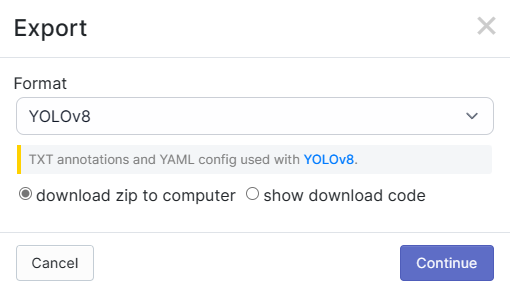
\includegraphics[width=.5\textwidth]{obrazky/roboflow/export.png}
        \caption{Exportovanie vytvoreného datasetu}
    \end{figure}

\chapter{Návrh softvéru}

    Pri návrhu a tvorbe aplikácie systému detekcie lietajúcich objektov bol kladený dôraz na:
    \begin{itemize}
        \item Spustiteľnosť a použiteľnosť na počítači
        \item Ovládateľnosť dotykovým panelom
        \item Modulárnosť a rozšíriteľnosť
        \item Spätná väzba a grafické zobrazenie výsledkov užívateľovi
        \item Možnosť používať, testovať a porovnávať rôzne metódy detekcie, klasifikácie a trasovania.
    \end{itemize}

    \section{Použitý jazyk a knižnice}

        Použitím programovacieho jazyka \emph{python}, bola získaná kompatibilita zo zariadeniami a operačnými systémami ktoré podporujú interpretér jazyka \emph{python}, teda hlavne \emph{Raspberry Pi} s nainštalovaným operačným systémom Raspberry Pi OS a osobné počítače, čo uľahčuje vývoj aplikácie a umožňuje jeho použitie na ľubovoľnom počítači.

        Na tvorbu grafického rozhrania bola použitá knižnica \ac{tkinter}. Tá umožňuje vytvárať grafické používateľské rozhranie priamo z kódu v jazyku \emph{python}. Obsahuje tiež objekty časovačov, vďaka ktorým je možné jednoducho a spoľahlivo ovládať kontinuálny beh aplikácie. Užívateľské rozhranie vytvorené knižnicou \ac{tkinter} je kompatibilné s ovládaním klávesnicou a myšou, aj dotykovým displejom.

        Knižnica \emph{OpenCV} obsahuje implementáciu množstva algorytmov spracovania obrazu a počítačového videnia. Umožňuje základné operácie s videom aj jednotlivými snímkami ako načítanie, ukladanie a zobrazovanie, pričom podporuje rôzne formáty obrazových dát. Sofistikovanejšie úlohy ktoré knižnica rieši zahrnujú detekciu, klasifikáciu, sledovanie pohybu. Knižnica \emph{OpenCV} je kompatibilná s viacerými programovacími jazykmi, vrátane jazyku \emph{python}.

    \section{Štruktúra aplikácie}

        Aplikácia je zložená z modulov reprezentujúcich jednotlivé implementované metódy detekcie, klasifikácie či trasovania alebo riadiacich modulov ovládajúcich tok dát medzi modulmi. Základnými typmi modulov tvoriacich aplikáciu sú:
        \begin{itemize}
            \item \textbf{Hlavná aplikácia} - existuje len jedna varianta, je zodpovedná za ovládanie systému, užívateľské rozhranie a súšťanie ostatných modulov. Pre každý z ďalších jednotlivých typov modulov je hlavnému modulu priradený zoznam existujúcich modulov daného typu, z ktorých si užívateľ môže vybrať ten aktívny, ktorý sa aktuálne použije na daný účel.
            \item \textbf{Poskytovateľ obrazu} - slúži na získavanie obrazových dát. Každý cyklus začína vyžiadaním nového obrazu od aktuálne zvoleného poskytovateľa obrazu hlavným modulom. Existujú dve varianty:
            \begin{itemize}
                \item \textbf{Video} - pri spustení aplikácia načíta všetky videá uložené v priečinku \path{./videos/} a pridá každému jeden objekt reprezentujúci dané video ako zdroj obrazu.
                \item \textbf{Kamera} - ak je v systéme nainštalovaná \emph{python} knižnica pre ovládanie kamery, je do zonamu poskytovateľov obrazu pridaný objekt reprezentujúci kameru.
            \end{itemize}
            \item \textbf{Detektor objektov} - po získaní aktuálneho obrazu je aplikovaný zvolený algorytmus detekcie. Detektoru je predaný obraz, jeho výstupom je zoznam rámikov oblastí v ktorých sa potenciálne nachádza objekt. V prípade zvolenia metódy detekcie a klasifikácie v jednom kroku je preskočený výber klasifikátora a výstupom je aj klasifikácia. 
            \item \textbf{Klasifikátor} - ak je zvolený algorytmus detekcie, sú oblasti s potenciálnym obsahom objektu predané klasifikátoru. Klasifikátor vráti hlavnému modulu zaradenie objektov do tried, po prípade označenie oblasti za pozadie. V hlavnej aplikácii je následne graficky zobrazené orámovanie a klasifikácia objektu.
            \item \textbf{Sledovač (Tracker)} - k ušetreniu výkonu je možne áplikovať detekciu a klasifikáciu len raz za určitý počet snímkov už a detekované a klasifikované objekty sledovať pomocou sledovačou z knižnice \emph{OpenCV}.
            \item \textbf{Tester výsledkov} - v prípade že je zvolené video ako zdroj obrazu a v priečinku \path{./video_annotation/} je pridaný \ac{csv} s rovnakým menom ako video obsahujúci správne orámovanie, je spustený testovací modul ktorý ohodnocuje detekciu a klasifikáciu podľa určenej správnej hodnoty zo súboru.
        \end{itemize}

        Jednotlivé moduly sú vytvárané dedením od abstraktnej triedy predstavujúcej rozhranie modulu s aplikáciou. Pre každý z typov modulu je pripravená jedna abstraktná rodičovská trieda, obsahujúca niektoré zdieľané premenné, ako je názov modulu a funkcie ktoré musí modul implementovať. Povinnou funkciou je napríklad funkcia vyžiadania si ďalšieho snímku pre modul poskytovateľa obrazu.

    \section{Implementácia}

        V aplikácii sú ako modul detekcie a klasifikácie aktuálne implementovaný model YOLO, pričom aplikácia automaticky pridá detekované naučené modely. Tie musia byť uložené v priečinku \path{./yolo/[model]/}, kde je \path{[model]} nahradené názvom modelu. v tomto priečinku je uložený model samotný v súbore \path{model.onnx} a \ac{csv} súbor so zoznamom názvov a farebných označení tried vo formáte \\
        \emph{"názov", "červená", "zelená", "modrá"} \\
        s názvom \path{classes.csv}. Aplikácia načíta všetky nájdené modely spolu s popisom tried a vloží ich do zoznamu detektorov.

    \section{Návrh grafického rozhrania}

        \ac{GUI} umožňuje intuitívne ovládanie aplikácie a zobrazovanie výsledkov detekcie, klasifikácie a sledovania.\linebreak Ovládanie jednotlivých modulov aplikácie je rozdelené do záložiek. Každá záložka umožňuje zvoliť ktorá z inštancii modulu každého z typov sa aktuálne používa.

        V ľavej časti obrazovky je zobrazený aktuálny snímok, s výstupom detekcie a klasifikácie. Zobrazujú sa v ňom orámovania detekovaných objektov, ich priradenie do tried a hodnotenie dôveryhodnosti klasifikácie. Ak existuje súbor s anotáciou správneho orámovania a klasifikácie pre aktuálne prehrávané video, sú zobrazené aj tie.

        V prvej záložke je užívateľovi umožnené zvoliť zdroj obrazu. Ak je aplikácia spustená na \emph{Raspberry Pi} a je nainštalovaná kižnica ovládania kamery, je do zoznamu zdrojov pridaná kamera. Pri spustení aplikácie sú načítané videá z priečinku \path{./videos} a sú zobrazené v zozname na záložke zdrojov spolu s kamerou. Kliknutím na názov zdroja je zdroj zvolený a užívateľovi sa z neho začne zobrazovať obraz.

        \begin{figure}[H]
            \centering
            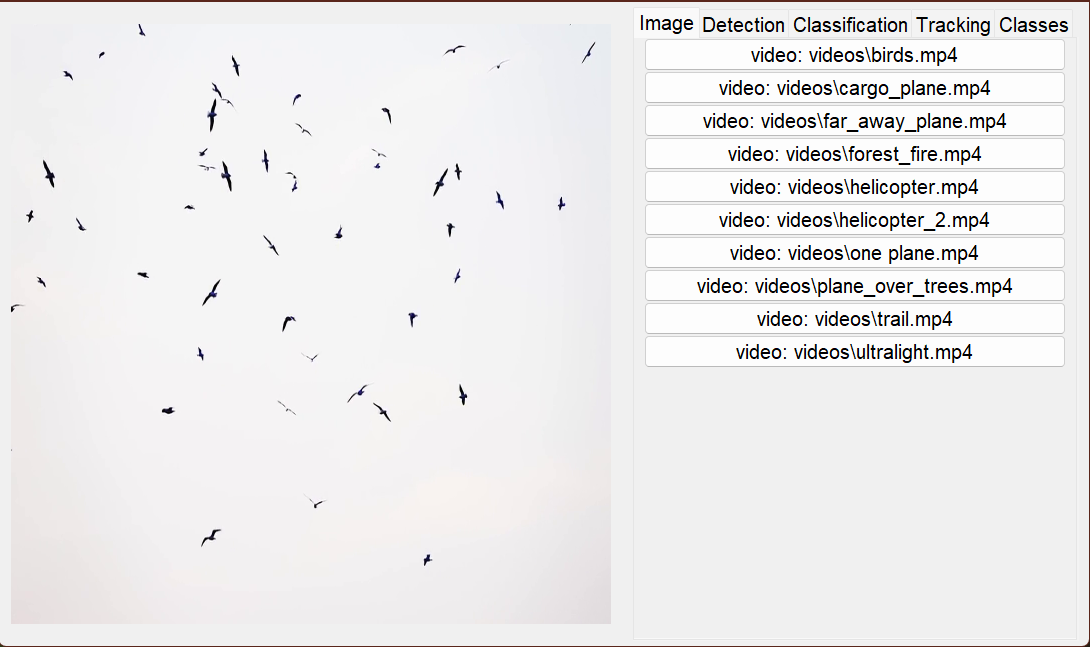
\includegraphics[width=.7\textwidth]{obrazky/app/image_provider.png}
            \caption{Záložka na výber poskytovateľa obrazu}
        \end{figure}

        V druhej záložke výberu detektora si užívateľ vyberie metódu detekcie, alebo metódu súčasnej detekcie a klasifikácie, pri ktorej nie je použiteľný výber klasifikátoru na ďalšej záložke. Zároveň je na tejto záložke nastaviteľná perióda spúšťania detekcie, medzi snímkami na ktorých je detekcia spustená sa buď zobrazované ohraničenie nemení, alebo je akutalizované sledovačom.

        \begin{figure}[H]
            \centering
            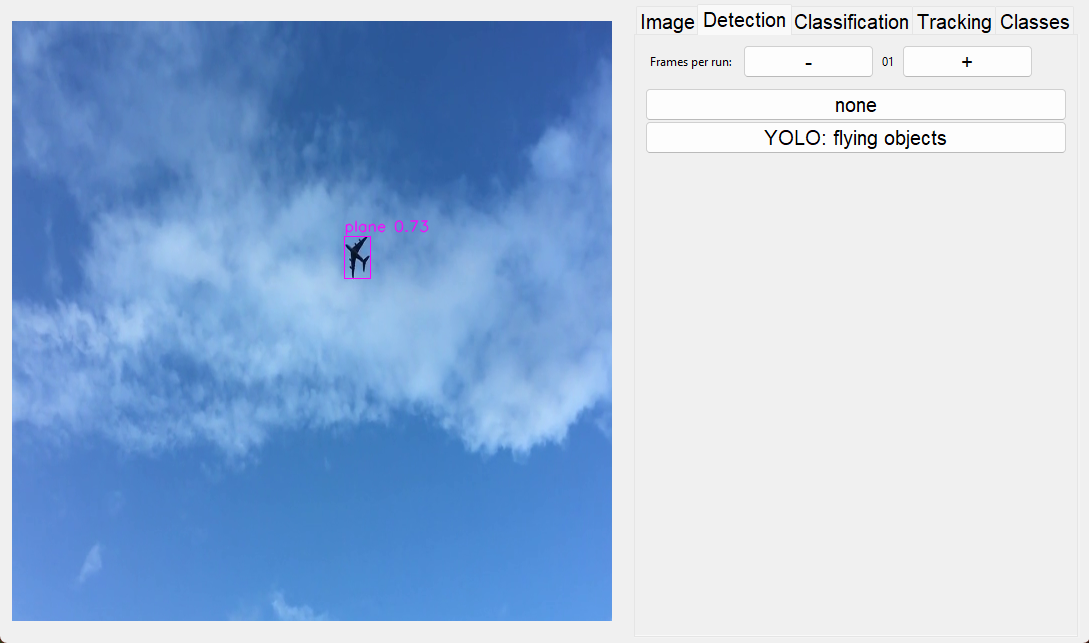
\includegraphics[width=.7\textwidth]{obrazky/app/detector.png}
            \caption{Záložka na výber metódy detekcie objektov}
        \end{figure}

        V záložke sledovania objektov je umiestnený výber zo sledovačov implementovaných v knižnici \emph{OpenCV}. Sledovač je použitý na snímkoch medzi spustením detektcie.

        \begin{figure}[H]
            \centering
            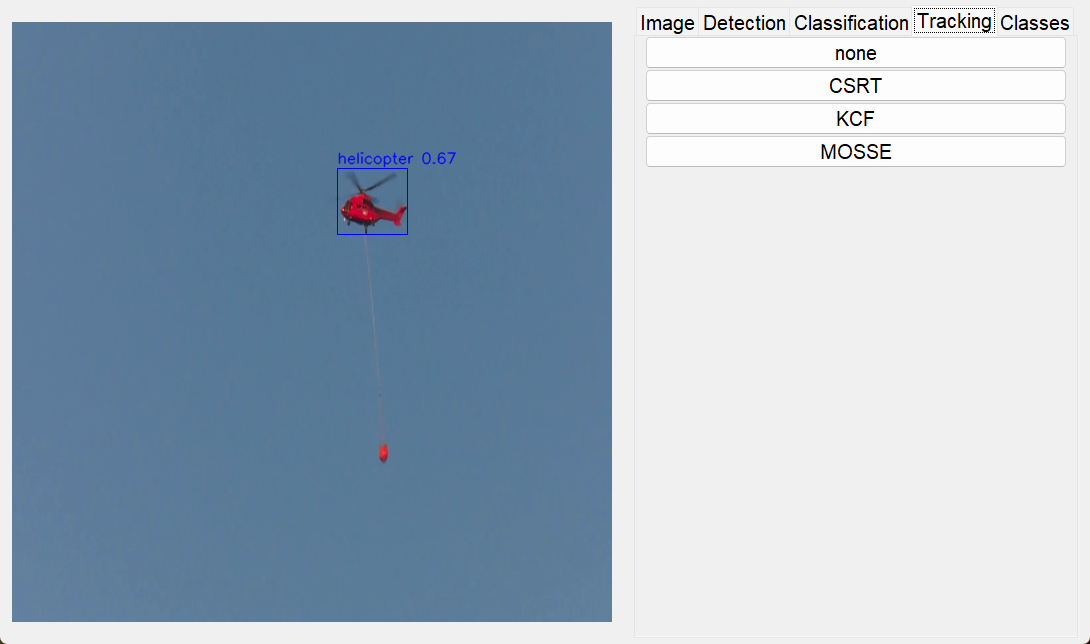
\includegraphics[width=.7\textwidth]{obrazky/app/tracker.png}
            \caption{Záložka na výber metódy sledovania objektov}
        \end{figure}

        Posledná záložka obsahuje menu z možnosťou zapnúť a vypnúť zobrazenie detekcie konkrétnych tried objektov. 

        \begin{figure}[H]
            \centering
            \begin{tikzpicture}[node distance=.5\textwidth]
                \node (image1) {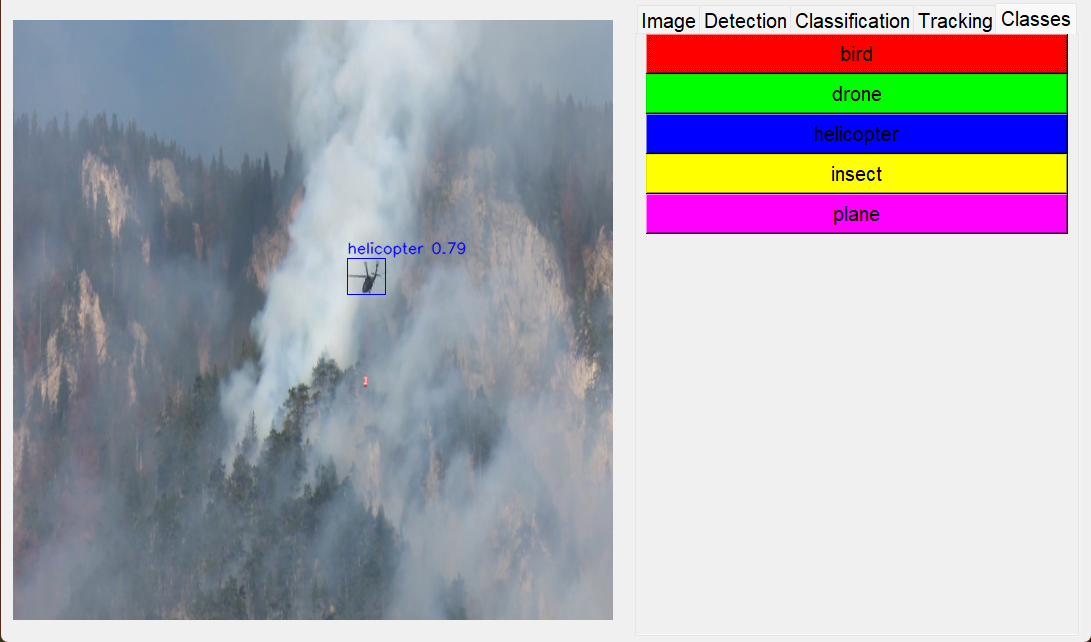
\includegraphics[width=.45\textwidth]{obrazky/app/class_settings_1.png}};
                \node (image2) [right of=image1] {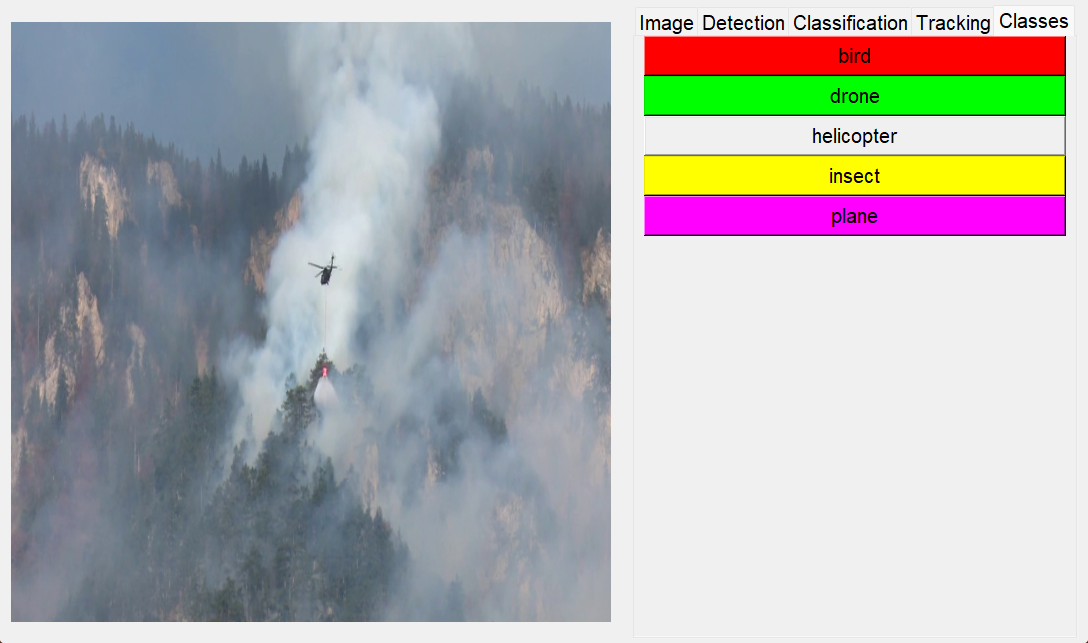
\includegraphics[width=.45\textwidth]{obrazky/app/class_settings_2.png}};
            \end{tikzpicture}
            \caption{Záložka na výber detekovaných tried}
        \end{figure}

%%% Vložení souboru 'text/vysledky' s popisem vysledků práce
% (rozdělte na více souborů či kapitol, pokud je vhodné)
\chapter{Výsledky studentské práce}

Praktická část a výsledky studentské práce vhodně rozdělené do částí.

\section{Programové řešení}
Lorem ipsum dolor sit amet, consectetuer adipiscing elit. Nulla pulvinar eleifend sem. Integer in sapien. Etiam sapien elit, consequat eget, tristique non, venenatis quis, ante. In laoreet, magna id viverra tincidunt, sem odio bibendum justo, vel imperdiet sapien wisi sed libero. Phasellus enim erat, vestibulum vel, aliquam a, posuere eu, velit. Aliquam erat volutpat. Nullam faucibus mi quis velit \cite{sr72/2017}.

\section{Výsledky měření}
Fusce tellus odio, dapibus id fermentum quis, suscipit id erat. Fusce tellus. Morbi scelerisque luctus velit. In laoreet, magna id viverra tincidunt, sem odio bibendum justo, vel imperdiet sapien wisi sed libero. Quisque porta. Fusce suscipit libero eget elit. Nulla non lectus sed nisl molestie malesuada. Phasellus faucibus molestie nisl. Integer vulputate sem a nibh rutrum consequat. Proin mattis lacinia justo. Phasellus et lorem id felis nonummy placerat. Etiam ligula pede, sagittis quis, interdum ultricies, scelerisque eu. Cras elementum. Aenean placerat. Donec ipsum massa, ullamcorper in, auctor et, scelerisque sed, est. Aliquam ante. Integer imperdiet lectus quis justo. Vivamus ac leo pretium faucibus. Nullam faucibus mi quis velit.

\subsection{Etiam quis quam}
Neque porro quisquam est, qui dolorem ipsum quia dolor sit amet, consectetur, adipisci velit, sed quia non numquam eius modi tempora incidunt ut labore et dolore magnam aliquam quaerat voluptatem. Aliquam erat volutpat. Lorem ipsum dolor sit amet, consectetuer adipiscing elit \cite{sr72/2017,pravidla}. Nunc auctor. Neque porro quisquam est, qui dolorem ipsum quia dolor sit amet, consectetur, adipisci velit, sed quia non numquam eius modi tempora incidunt ut labore et dolore magnam aliquam quaerat voluptatem. Maecenas lorem. Maecenas libero. In laoreet, magna id viverra tincidunt, sem odio bibendum justo, vel imperdiet sapien wisi sed libero. Nullam rhoncus aliquam metus.

\subsubsection{Integer rutrum orci vestibulum}
Integer rutrum, orci vestibulum ullamcorper ultricies, lacus quam ultricies odio, vitae placerat pede sem sit amet enim. Ut enim ad minim veniam, quis nostrud exercitation ullamco laboris nisi ut aliquip ex ea commodo consequat. Fusce tellus odio, dapibus id fermentum quis, suscipit id erat. Nullam eget nisl. Nunc auctor. Etiam dui sem, fermentum vitae, sagittis id, malesuada in, quam. Fusce dui leo, imperdiet in, aliquam sit amet, feugiat eu, orci. Curabitur vitae diam non enim vestibulum interdum. Aliquam erat volutpat. Pellentesque sapien. Phasellus enim erat, vestibulum vel, aliquam a, posuere eu, velit.

\subsubsection{Eger rutrum orci westibulum}
Fusce dui leo, imperdiet in, aliquam sit amet, feugiat eu, orci. Maecenas aliquet accumsan leo. Aliquam ornare wisi eu metus. Cum sociis natoque penatibus et magnis dis parturient montes, nascetur ridiculus mus. Aliquam erat volutpat. Donec iaculis gravida nulla. Sed elit dui, pellentesque a, faucibus vel, interdum nec, diam. Temporibus autem quibusdam et aut officiis debitis aut rerum necessitatibus saepe eveniet ut et voluptates repudiandae sint et molestiae non recusandae. Nulla non arcu lacinia neque faucibus fringilla. Phasellus enim erat, vestibulum vel, aliquam a, posuere eu, velit. Praesent vitae arcu tempor neque lacinia pretium
\cite{Walter1999,Svacina1999IEEE,RajmicSysel2002}.

Aliquam erat volutpat. Quisque porta. Integer imperdiet lectus quis justo. Nullam justo enim, consectetuer nec, ullamcorper ac, vestibulum in, elit. Nullam faucibus mi quis velit. Fusce tellus. Fusce consectetuer risus a nunc. Cras pede libero, dapibus nec, pretium sit amet, tempor quis. Morbi imperdiet, mauris ac auctor dictum, nisl ligula egestas nulla, et sollicitudin sem purus in lacus
\cite{CSN_ISO_690-2022,CSN_ISO_7144-1997,CSN_ISO_31-11}.
Mauris elementum mauris vitae tortor. Neque porro quisquam est, qui dolorem ipsum quia dolor sit amet, consectetur, adipisci velit, sed quia non numquam eius modi tempora incidunt ut labore et dolore magnam aliquam quaerat voluptatem. Quisque porta. Integer vulputate sem a nibh rutrum consequat. Nulla pulvinar eleifend sem. Praesent id justo in neque elementum ultrices \cite{Farkasova23:CSNISO6902022komentar}.

Fusce suscipit libero eget elit. Integer vulputate sem a nibh rutrum consequat. Aliquam erat volutpat. Etiam neque. Nulla turpis magna, cursus sit amet, suscipit a, interdum id, felis. Nullam rhoncus aliquam metus. Etiam dui sem, fermentum vitae, sagittis id, malesuada in, quam. Nunc auctor. Nunc dapibus tortor vel mi dapibus sollicitudin. Praesent in mauris eu tortor porttitor accumsan. Nulla non arcu lacinia neque faucibus fringilla. Nullam lectus justo, vulputate eget mollis sed, tempor sed magna. Maecenas lorem. Aenean placerat. Donec vitae arcu. Maecenas lorem. Donec iaculis gravida nulla. Nulla non lectus sed nisl molestie malesuada.

Duis pulvinar. Nulla est. Duis condimentum augue id magna semper rutrum. Integer pellentesque quam vel velit. Aliquam ante. Nulla quis diam. Proin mattis lacinia justo. Aenean fermentum risus id tortor. Nunc auctor. Nullam justo enim, consectetuer nec, ullamcorper ac, vestibulum in, elit. In dapibus augue non sapien. Etiam bibendum elit eget erat. In sem justo, commodo ut, suscipit at, pharetra vitae, orci. Maecenas libero.

Nulla non lectus sed nisl molestie malesuada. Donec vitae arcu. Aenean fermentum risus id tortor. Praesent in mauris eu tortor porttitor accumsan. Nulla pulvinar eleifend sem. Duis viverra diam non justo. Integer imperdiet lectus quis justo. Pellentesque habitant morbi tristique senectus et netus et malesuada fames ac turpis egestas. In rutrum. Excepteur sint occaecat cupidatat non proident, sunt in culpa qui officia deserunt mollit anim id est laborum. Nulla non lectus sed nisl molestie malesuada. Aliquam erat volutpat. Mauris tincidunt sem sed arcu. Duis bibendum, lectus ut viverra rhoncus, dolor nunc faucibus libero, eget facilisis enim ipsum id lacus. Fusce tellus odio, dapibus id fermentum quis, suscipit id erat. In enim a arcu imperdiet malesuada. Nulla non lectus sed nisl molestie malesuada. Proin mattis lacinia justo.

Aliquam in lorem sit amet leo accumsan lacinia. Cum sociis natoque penatibus et magnis dis parturient montes, nascetur ridiculus mus. Duis sapien nunc, commodo et, interdum suscipit, sollicitudin et, dolor. Suspendisse sagittis ultrices augue. Nullam lectus justo, vulputate eget mollis sed, tempor sed magna. In convallis. Praesent id justo in neque elementum ultrices. Neque porro quisquam est, qui dolorem ipsum quia dolor sit amet, consectetur, adipisci velit, sed quia non numquam eius modi tempora incidunt ut labore et dolore magnam aliquam quaerat voluptatem.

Pellentesque pretium lectus id turpis. Nemo enim ipsam voluptatem quia voluptas sit aspernatur aut odit aut fugit, sed quia consequuntur magni dolores eos qui ratione voluptatem sequi nesciunt. Curabitur ligula sapien, pulvinar a vestibulum quis, facilisis vel sapien. Praesent dapibus. Sed elit dui, pellentesque a, faucibus vel, interdum nec, diam. Duis viverra diam non justo. Duis ante orci, molestie vitae vehicula venenatis, tincidunt ac pede. Phasellus rhoncus. Maecenas fermentum, sem in pharetra pellentesque, velit turpis volutpat ante, in pharetra metus odio a lectus. Proin pede metus, vulputate nec, fermentum fringilla, vehicula vitae, justo. Fusce aliquam vestibulum ipsum. Nullam at arcu a est sollicitudin euismod.

%Aliquam ante. Phasellus faucibus molestie nisl. Etiam ligula pede, sagittis quis, interdum ultricies, scelerisque eu. Morbi leo mi, nonummy eget tristique non, rhoncus non leo. Cum sociis natoque penatibus et magnis dis parturient montes, nascetur ridiculus mus. Morbi scelerisque luctus velit. Curabitur bibendum justo non orci. Donec quis nibh at felis congue commodo. Nullam faucibus mi quis velit. Aenean id metus id velit ullamcorper pulvinar. Pellentesque sapien. Fusce nibh. Vestibulum fermentum tortor id mi. Nullam eget nisl. Praesent vitae arcu tempor neque lacinia pretium. Proin in tellus sit amet nibh dignissim sagittis. Donec quis nibh at felis congue commodo.
%
%Nam quis nulla. Proin in tellus sit amet nibh dignissim sagittis. Nullam dapibus fermentum ipsum. Curabitur ligula sapien, pulvinar a vestibulum quis, facilisis vel sapien. Nam libero tempore, cum soluta nobis est eligendi optio cumque nihil impedit quo minus id quod maxime placeat facere possimus, omnis voluptas assumenda est, omnis dolor repellendus. Vivamus ac leo pretium faucibus. Nunc tincidunt ante vitae massa. Maecenas sollicitudin. Ut tempus purus at lorem. Nullam lectus justo, vulputate eget mollis sed, tempor sed magna. Fusce consectetuer risus a nunc. Etiam quis quam.
%
%Donec quis nibh at felis congue commodo. Sed vel lectus. Donec odio tempus molestie, porttitor ut, iaculis quis, sem. Nullam feugiat, turpis at pulvinar vulputate, erat libero tristique tellus, nec bibendum odio risus sit amet ante. Sed elit dui, pellentesque a, faucibus vel, interdum nec, diam. Cras elementum. Sed vel lectus. Donec odio tempus molestie, porttitor ut, iaculis quis, sem. Etiam neque. Integer tempor. Vivamus porttitor turpis ac leo. Nulla non arcu lacinia neque faucibus fringilla.
%
%Etiam posuere lacus quis dolor. Nemo enim ipsam voluptatem quia voluptas sit aspernatur aut odit aut fugit, sed quia consequuntur magni dolores eos qui ratione voluptatem sequi nesciunt. Nullam faucibus mi quis velit. Cum sociis natoque penatibus et magnis dis parturient montes, nascetur ridiculus mus. Phasellus faucibus molestie nisl. Maecenas ipsum velit, consectetuer eu lobortis ut, dictum at dui. Maecenas aliquet accumsan leo. Pellentesque ipsum. Donec vitae arcu. Suspendisse nisl. Morbi imperdiet, mauris ac auctor dictum, nisl ligula egestas nulla, et sollicitudin sem purus in lacus. Pellentesque ipsum. Ut enim ad minima veniam, quis nostrum exercitationem ullam corporis suscipit laboriosam, nisi ut aliquid ex ea commodi consequatur? Nam libero tempore, cum soluta nobis est eligendi optio cumque nihil impedit quo minus id quod maxime placeat facere possimus, omnis voluptas assumenda est, omnis dolor repellendus.


%%% Vložení souboru 'text/zaver' se závěrem
\chapter*{Záver}
\phantomsection
\addcontentsline{toc}{chapter}{Závěr}

% Shrnutí studentské práce.

V~tejto práci bol popísaný návrh systému detekcie, trasovania a~klasifikácie lietajúcich objektov. V~kapitolách teoretickej časti práce boli vysvetlené teoretické základy postupov a~metód detekcie objektov v~obraze, ich popisu a~následného zaradenia do~tried. Dôraz bol kladený na~rozdiely medzi metódami, ich výhody a~nevýhody.

Nasledujúce kapitoly sa~venovali samotnému návrhu systému. Bol navrhnutý a~odôvodnený výber hardvérových komponentov a~ich prepojenie. Pre jednoduchosť, spoľahlivosť a~dostatočný výkon bola zvolená platforma \emph{Raspberry Pi} s~dotykovým panelom ako užívateľským rozhraním a~kamerou od~spoločnosti \emph{Raspberry}.

Ďalej bol zdokumentovaný návrh databázy anotovaných snímkov určených na~trénovanie klasifikátorov. Pri vytváraní bol použitý program \emph{roboflow}. Výsledná databáza vznikla spojením datasetu z~práce~\cite{Jurecka2021}, niekoľkých voľne dostupných datasetov spolu s~osobne získanými a~anotovanými fotografiami. Správnosť takto získanej databázy bola overená naučením modelu v~systéme \emph{roboflow} v~nastavení na~odskúšanie (fast). Na testovacej množine tento model dosahoval úroveň~\ac{mAP}~86,1~\%.

Nakoniec bol popísaný softvér pre~navrhovaný systém, jeho štruktúra a~implementácia jeho častí. Spomenuté boli nástroje~a knižnice použité pri~jeho vývoji. Softvér zahrňuje moduly pre~výber zdroja dát, detekciu objektov, ich klasifikáciu, sledovanie a~kontrolu presnosti porovnaním s~anotáciou. Systém umožňuje výber aktuálne používanej metódy a~porovnanie medzi metódami. Keďže bol použitý programovací jazyk \emph{python} a knižnice dostupné na väčšine zariadení a operačných systémoch, je možné program spustiť aj na~bežnom počítači.

Ciele pokračovania tejto práce zahřňujú ďalšie rozširovanie datasetu, implementáciu viacerých metód detekcie~a klasifikácie a vyhodnotenie a porovnanie prístupov.

%%% Vložení souboru 'text/literatura' se seznamem zdrojů
% Pro sazbu seznamu literatury použijte jednu z následujících možností

%%%%%%%%%%%%%%%%%%%%%%%%%%%%%%%%%%%%%%%%%%%%%%%%%%%%%%%%%%%%%%%%%%%%%%%%%
%1) Seznam citací definovaný přímo pomocí prostředí literatura / thebibliography

\begin{thebibliography}{99}
	
	\bibitem{Jurecka2021} % predošlá diplomová práca
		JUREČKA, Tomáš. Detekce a klasifikace létajících objektů. Brno, 2021. Diplomová práca.

	\bibitem{Janousek2018} % Algoritmy detekcie lietajúcich objektov, príspevok PIERS
		JANOUŠEK, Jiří, Jan NOVOTNÝ, Petr MARCOŇ a Anna SIRUCKOVA. Algorithms for Flying Object Detection. In: 2018 Progress In Electromagnetics Research Symposium (PIERS-Toyama) [online]. Toyma, Japonsko, 2018, s. 782-783 [cit. 2024-01-03]. ISBN 978-4-8855-2316-8. ISSN 1559-9450. Dostupné z: doi:10.23919/PIERS.2018.8598196

	\bibitem{Morse1998/1} % Prahovanie, prednáška online
		MORSE, Bryan. Lecture 4: Thresholding [online]. Brigham, 1998 [cit. 2024-01-03]. Dostupné z: \url{https://homepages.inf.ed.ac.uk/rbf/CVonline/LOCAL_COPIES/MORSE/threshold.pdf}. Brigham Young University.

	\bibitem{Morse1998/2} % Popis objektu - radiometrické deskriptory, prednáška online
		MORSE, Bryan. Lecture 9: Shape Description (Regions) [online]. Brigham, 1998 [cit. 2024-01-03]. Dostupné z: \url{https://homepages.inf.ed.ac.uk/rbf/CVonline/LOCAL_COPIES/MORSE/region-props-and-moments.pdf}. Brigham Young University.

	\bibitem{Buhl2023} % Prahovanie, web online
		BUHL, Nikolaj. Image Thresholding in Image Processing. Encord [online]. 2023 [cit. 2024-01-03]. Dostupné z: \url{https://encord.com/blog/image-thresholding-image-processing/}

	\bibitem{Samina2023} % Cannyho detektor, web online
		SAMINA. EDUCATIVE, INC. What is Canny edge detection? EDUCATIVE, INC. Educative [online]. Educative, 2023 [cit. 2024-01-03]. Dostupné z: \url{https://www.educative.io/answers/what-is-canny-edge-detection}

	\bibitem{OpenCV2023} % Odčítanie pozadia, dokumentácia OpenCV
		OPEN SOURCE COMPUTER VISION. How to Use Background Subtraction Methods [online]. 2023 [cit. 2024-01-03]. Dostupné z: \url{https://docs.opencv.org/4.x/d1/dc5/tutorial_background_subtraction.html}

	\bibitem{Leung2021} % Kreslenie CNN, web online
		LEUNG, Kenneth. How to Easily Draw Neural Network Architecture Diagrams [online]. In: . [cit. 2024-01-03]. Dostupné z: \url{https://towardsdatascience.com/how-to-easily-draw-neural-network-architecture-diagrams-a6b6138ed875}

	\bibitem{Erbo2017} % Geometrické momenty a invarianty, článok online
		LI, Erbo, Yazhou HUANG, Dong XU a Hua LI. Shape DNA: Basic Generating Functions for Geometric Moment Invariants [online]. Cornell University, 2017, 3-8 [cit. 2024-01-03]. Dostupné z: doi:10.48550/arXiv.1703.02242

	\bibitem{Wood2011} % How High Birds Fly I
		LI, Erbo, Yazhou HUANG, Dong XU a Hua LI. Shape DNA: Basic Generating Functions for Geometric Moment Invariants [online]. Cornell University, 2017, 3-8 [cit. 2024-01-03]. Dostupné z: doi:10.48550/arXiv.1703.02242
% \bibitem{sr72/2017}
% 	VYSOKÉ UČENÍ TECHNICKÉ V~BRNĚ.
% 	\emph{Směrnice č.\,72/2017, Úprava, odevzdávání a~zveřejňování závěrečných prací.}
% 	Online. Brno: VUT v~Brně, 2017.
% 	Úplné znění ke dni 11.\,4.\,2022.
% 	Dostupné z:\\
% 	{\small
% 	\url{https://www.vut.cz/uredni-deska/vnitrni-predpisy-a-dokumenty/smernice-c-72-2017-uprava-odevzdavani-a-zverejnovani-zaverecnych-praci-d161410}.}
% 	[cit.\ 2023-09-27].
%  
%  \bibitem{CSN_ISO_690-2022}
%      ÚŘAD PRO TECHNICKOU NORMALIZACI, METROLOGII A~STÁTNÍ ZKUŠEBNICTVÍ.
%      ČSN ISO 690:2022 (01 0197), \emph{Informace a dokumentace -- Pravidla pro bibliografické odkazy a~citace informačních zdrojů.}
%      Čtvrté vydání. Praha, 2022.
%  
%  \bibitem{CSN_ISO_7144-1997}
%      ÚŘAD PRO TECHNICKOU NORMALIZACI, METROLOGII A~STÁTNÍ ZKUŠEBNICTVÍ.
%      ČSN ISO 7144 (010161), \emph{Dokumentace -- Formální úprava disertací a~podobných dokumentů.}
%  %    24 stran.
%      Praha, 1997.
%  
%  \bibitem{CSN_ISO_31-11}
%      ÚŘAD PRO TECHNICKOU NORMALIZACI, METROLOGII A~STÁTNÍ ZKUŠEBNICTVÍ.
%      ČSN ISO 31-11, \emph{Veličiny a~jednotky -- část 11: Matematické znaky a~značky používané ve fyzikálních vědách a~v~technice.}
%      Praha, 1999.
%  
%  \bibitem{Farkasova23:CSNISO6902022komentar}
%  	FARKAŠOVÁ, B. et al.
%  	\emph{Výklad normy ČSN ISO 690:2022 (01 0197) účinné od 1.\,12.\,2022}.
%  	 Online. První vydání. 2023.
%  	Dostupné~z:
%  	\url{https://www.citace.com/Vyklad-CSN-ISO-690-2022.pdf}.
%  	[cit.\,2023-09-27].
%  
%  \bibitem{pravidla}
%      \emph{Pravidla českého pravopisu}.
%  	1.\ vydání. Olomouc: FIN, 1998.\\
%  	\mbox{ISBN 80-86002-40-3}.
%  
%  \bibitem{Walter1999}
%  	WALTER, G.\,G. a SHEN, X.
%  	\emph{Wavelets and Other Orthogonal Systems}.
%  	2.\,vydání, Boca Raton: Chapman\,\&\,Hall/CRC, 2000.
%  	ISBN 1-58488-227-1
%  
%  \bibitem{Svacina1999IEEE}
%  	SVAČINA, J.
%  	Dispersion Characteristics of Multilayered Slotlines -- a Simple Approach.
%  	\emph{IEEE Transactions on Microwave Theory and Techniques}.
%  	1999, vol.\,47, no.\,9, s.\,1826--1829. ISSN 0018-9480.
%  
%  \bibitem{RajmicSysel2002}
%      RAJMIC, P. a SYSEL, P.
%      Wavelet Spectrum Thresholding Rules.
%      In: \emph{Proceedings of the International Conference Research in Telecommunication Technology}.
%      Žilina: Žilina University, 2002. s.\,60--63. ISBN 80-7100-991-1.
%  
\end{thebibliography}


%%%%%%%%%%%%%%%%%%%%%%%%%%%%%%%%%%%%%%%%%%%%%%%%%%%%%%%%%%%%%%%%%%%%%%%%%
%%2) Seznam citací pomocí BibTeXu
%% Při použití je nutné v TeXnicCenter ve výstupním profilu aktivovat spouštění BibTeXu po překladu.
%% Definice stylu seznamu
%\bibliographystyle{unsrturl}
%% Pro českou sazbu lze použít styl czechiso.bst ze stránek
%% http://www.fit.vutbr.cz/~martinek/latex/czechiso.tar.gz
% \bibliographystyle{Czech}
%% Vložení souboru se seznamem citací
% \bibliography{text/literatura}
%
%% Následující příkaz je pouze pro ukázku sazby literatury při použití BibTeXu.
%% Způsobí citaci všech zdrojů v souboru literatura.bib, i když nejsou citovány v textu.
% \nocite{*}

%%% Vložení souboru 'text/zkratky' se seznam použitých symbolů, veličin a zkratek
\cleardoublepage
\chapter*{\listofabbrevname}
\phantomsection
\addcontentsline{toc}{chapter}{\listofabbrevname}

\begin{acronym}[KolikMista]

	\acro{ReLU}
		[ReLU]
		{Usmernená lineárna jednotka}

	\acro{CNN}
		[CNN]
		{Konvolučné neurónové siete (Convolutional neural network)}

	\acro{R-CNN}
		[R-CNN]
		{Konvolučné neurónové siete založené na regiónoch (Region-based CNN)}

	\acro{RoI}
		[RoI]
		{Regióny záujmu (Regions of Interest)}

	\acro{SVM}
		[SVM]
		{Metódy podporných vektorov (Support Vector Machine)}

	\acro{RPN}
		[RPN]
		{Sieť návrhu regiónov (Region Proposal Network)}

	\acro{YOLO}
		[YOLO]
		{You only look once}
	
	\acro{IOU}
		[IOU]
		{Pomer prieniku voči zjednoteniu (Intersection over Union)}
	
	\acro{tkinter}
		[tkinter]
		{Rozhranie toolkitu Tcl/Tk (Tk interface)}

	\acro{csv}
		[csv]
		{Súbor s čiarkou rozdelenými hodnotami (Comma Separated Values)}

	\acro{GUI}
		[GUI]
		{Grafické užívateľské rozhranie (Graphical User Interface)}

	\acro{mAP}
		[mAP]
		{Stredná priemerná presnosť (Mean Average Precision)}

	% \acro{zkTemp}		% název
	% 	[Šířka levého sloupce Seznamu symbolů a zkratek]								% zkratka
	% 	{je určena šířkou parametru prostředí \texttt{acronym} (viz řádek~1 výpisu zdrojáku na~str.\,\pageref{lst:zkratky})}
	% 										% rozvinutí zkratky

	% \acro{zkDummy}
	% 	[KolikMista]
	% 	{pouze ukázka vyhrazeného místa}

	% \acro{DSP}		% název/zkratka
	% 	{číslicové zpracování signálů -- Digital Signal Processing}
	% 										% rozvinutí zkratky
	% %%% bsymfvz
	% \acro{symfvz}						% název
	% 	[\ensuremath{f_\textind{vz}}] % symbol
	% 	{vzorkovací kmitočet}					% popis
	% %%% esymfvz

\end{acronym}


%%% Začátek příloh
\appendix

%%% Vysázení seznamu příloh
% (vynechejte, pokud máte dvě nebo méně příloh)
\listofappendices

%%% Vložení souboru 'text/prilohy' s přílohami
% Obvykle je přítomen alespoň popis co najdeme na přiloženém médiu
\chapter{Některé příkazy balíčku \texttt{thesis}}

\section{Příkazy pro sazbu veličin a jednotek}

\begin{table}[!h]
  \caption[Přehled příkazů]{Přehled příkazů pro matematické prostředí }
  \begin{center}
  	\small
	  \begin{tabular}{|c|c|c|c|}
	    \hline
	    Příkaz    						& Příklad 					& Zdroj příkladu  							& Význam  \\
	    \hline\hline
	    \verb|\textind{...}|	& $\beta_\textind{max}$ 	& \verb|$\beta_\textind{max}$|	& textový index \\
	    \hline
	    \verb|\const{...}| 		& $\const{U}_\textind{in}$ 				& \verb|$\const{U}_\textind{in}$|		& konstantní veličina \\
	    \hline
	    \verb|\var{...}| 		& $\var{u}_\textind{in}$ & \verb|$\var{u}_\textind{in}$| & proměnná veličina \\
	    \hline
	    \verb|\complex{...}| 	& $\complex{u}_\textind{in}$ & \verb|$\complex{u}_\textind{in}$| & komplexní veličina \\
	    \hline
	    \verb|\vect{...}| 		& $\vect{y}$ 						& \verb|$\vect{y}$| & vektor \\
	    \hline
	    \verb|\mat{...}| 	& $\mat{Z}$ 						& \verb|$\mat{Z}$| & matice \\
	    \hline
	    \verb|\unit{...}| 		& $\unit{kV}$ 						& \verb|$\unit{kV}$|\quad či\ \, \verb|\unit{kV}| & jednotka \\
	    \hline
	  \end{tabular}
  \end{center}
\end{table}



%\newpage
\section{Příkazy pro sazbu symbolů}

\begin{itemize}
  \item
    \verb|\E|, \verb|\eul| -- sazba Eulerova čísla: $\eul$,
  \item
    \verb|\J|, \verb|\jmag|, \verb|\I|, \verb|\imag| -- sazba imaginární jednotky: $\jmag$, $\imag$,
  \item
    \verb|\dif| -- sazba diferenciálu: $\dif$,
  \item
    \verb|\sinc| -- sazba funkce: $\sinc$,
  \item
    \verb|\mikro| -- sazba symbolu mikro stojatým písmem%
			\footnote{znak pochází z~balíčku \texttt{textcomp}}: $\mikro$,
	\item
		\verb|\uppi| -- sazba symbolu $\uppi$
			(stojaté řecké pí, na rozdíl od \verb|\pi|, což sází $\pi$).
\end{itemize}
%
Všechny symboly jsou určeny pro matematický mód, vyjma \verb|\mikro|, jenž je\\ použitelný rovněž v~textovém módu.
%$\upmikro$


\chapter{Druhá příloha}

\begin{figure}[!h]
  \begin{center}
    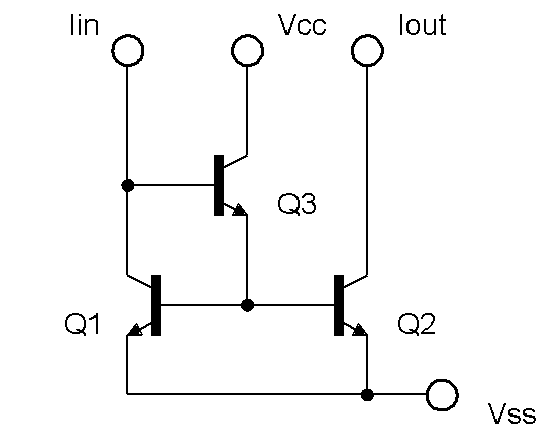
\includegraphics[scale=0.5]{obrazky/ZlepseneWilsonovoZrcadloNPN}
  \end{center}
  \caption[Alenčino zrcadlo]{Zlepšené Wilsonovo proudové zrcadlo.}
\end{figure}

Pro sazbu vektorových obrázků přímo v~\LaTeX{}u je možné doporučit balíček \href{https://www.ctan.org/pkg/pgf}{\texttt{TikZ}}.
Příklady sazby je možné najít na \href{http://www.texample.net/tikz/examples/}{\TeX{}ample}.
Pro vyzkoušení je možné použít programy QTikz nebo TikzEdt.




\chapter{Příklad sazby zdrojových kódů}

\section{Balíček \texttt{listings}}

Pro vysázení zdrojových souborů je možné použít balíček \href{https://www.ctan.org/pkg/listings}{\texttt{listings}}.
Balíček zavádí nové prostředí \texttt{lstlisting} pro sazbu zdrojových kódů, jako například:
%
\begin{lstlisting}[language={[LaTeX]TeX}]
\section{Balíček lstlistings}
Pro vysázení zdrojových souborů je možné použít
	balíček \href{https://www.ctan.org/pkg/listings}%
	{\texttt{listings}}.
Balíček zavádí nové prostředí \texttt{lstlisting} pro
	sazbu zdrojových kódů.
\end{lstlisting}
%
Podporuje množství programovacích jazyků.
Kód k~vysázení může být načítán přímo ze zdrojových souborů.
Umožňuje vkládat čísla řádků nebo vypisovat jen vybrané úseky kódu.
Např.:

\noindent
Zkratky jsou sázeny v~prostředí \texttt{acronym}:
\label{lst:zkratky}
\lstinputlisting[language={[LaTeX]TeX},nolol,numbers=left, firstnumber=6, firstline=6,lastline=6]{text/zkratky.tex}
%
Šířka textu volitelného parametru \verb|KolikMista| udává šířku prvního sloupce se zkratkami.
Proto by měla být zadávána nejdelší zkratka nebo symbol.
Příklad definice zkratky \acs{symfvz} je na výpisu \ref{lst:symfvz}.

\shorthandoff{-}
\lstinputlisting[language={[LaTeX]TeX},frame=single,caption={Ukázka sazby zkratek},label=lst:symfvz,numbers=left,linerange={bsymfvz-\%\%\%\ esymfvz},includerangemarker=false]{text/zkratky.tex}
\shorthandon{-}

\noindent
Ukončení seznamu je provedeno ukončením prostředí:
\lstinputlisting[language={[LaTeX]TeX},nolol,numbers=left,firstnumber=26,linerange=26]{text/zkratky.tex}

\vspace{\fill}

\noindent
{\bf Poznámka k~výpisům s~použitím volby jazyka \verb|czech| nebo \verb|slovak|:}\newline
Pokud Váš zdrojový kód obsahuje znak spojovníku \verb|-|, pak překlad může skončit chybou.
Ta je způsobená tím, že znak \verb|-| je v~českém nebo slovenském nastavení balíčku \verb|babel| tzv.\ aktivním znakem.
Přepněte znak \verb|-| na neaktivní příkazem \verb|\shorthandoff{-}| těsně před výpisem a hned za ním jej vraťte na aktivní příkazem \verb|\shorthandon{-}|.
Podobně jako to je ukázáno ve zdrojovém kódu šablony.


\clearpage

%\section{Výpis kódu prostředí Matlab}
Na výpisu \ref{lst:priklad.vypis.kodu.Matlab} naleznete příklad kódu pro Matlab, na výpisu \ref{lst:priklad.vypis.kodu.C} zase pro jazyk~C.

\lstnewenvironment{matlab}[1][]{%
\iflanguage{czech}{\shorthandoff{-}}{}%
\iflanguage{slovak}{\shorthandoff{-}}{}%
\lstset{language=Matlab,numbers=left,#1}%
}{%
\iflanguage{slovak}{\shorthandon{-}}{}%
\iflanguage{czech}{\shorthandon{-}}{}%
}

\begin{matlab}[frame=single,float=htbp,caption={Příklad Schur-Cohnova testu stability v~prostředí Matlab.},label=lst:priklad.vypis.kodu.Matlab,numberstyle=\scriptsize, numbersep=7pt]
%% Priklad testovani stability filtru

% koeficienty polynomu ve jmenovateli
a = [ 5, 11.2, 5.44, -0.384, -2.3552, -1.2288];
disp( 'Polynom:'); disp(poly2str( a, 'z'))

disp('Kontrola pomoci korenu polynomu:');
zx = roots( a);
if( all( abs( zx) < 1))
    disp('System je stabilni')
else
    disp('System je nestabilni nebo na mezi stability');
end

disp(' '); disp('Kontrola pomoci Schur-Cohn:');
ma = zeros( length(a)-1,length(a));
ma(1,:) = a/a(1);
for( k = 1:length(a)-2)
    aa = ma(k,1:end-k+1);
    bb = fliplr( aa);
    ma(k+1,1:end-k+1) = (aa-aa(end)*bb)/(1-aa(end)^2);
end

if( all( abs( diag( ma.'))))
    disp('System je stabilni')
else
    disp('System je nestabilni nebo na mezi stability');
end
\end{matlab}

\noindent
\begin{minipage}{\linewidth}


%\section{Výpis kódu jazyka C}

\begin{lstlisting}[frame=single,numbers=right,caption={Příklad implementace první kanonické formy v~jazyce C.},label=lst:priklad.vypis.kodu.C,basicstyle=\ttfamily\small, keywordstyle=\color{black}\bfseries\underbar,]
// první kanonická forma
short fxdf2t( short coef[][5], short sample)
{
	static int v1[SECTIONS] = {0,0},v2[SECTIONS] = {0,0};
	int x, y, accu;
	short k;

	x = sample;
	for( k = 0; k < SECTIONS; k++){
		accu = v1[k] >> 1;
		y = _sadd( accu, _smpy( coef[k][0], x));
		y = _sshl(y, 1) >> 16;

		accu = v2[k] >> 1;
		accu = _sadd( accu, _smpy( coef[k][1], x));
		accu = _sadd( accu, _smpy( coef[k][2], y));
		v1[k] = _sshl( accu, 1);

		accu = _smpy( coef[k][3], x);
		accu = _sadd( accu, _smpy( coef[k][4], y));
		v2[k] = _sshl( accu, 1);

		x = y;
	}
	return( y);
}
\end{lstlisting}
\end{minipage}







\chapter{Obsah elektronické přílohy}
Elektronická příloha je často nedílnou součástí semestrální nebo závěrečné práce.
Vkládá se do informačního systému VUT v~Brně ve vhodném formátu (ZIP, PDF\,\dots).

Nezapomeňte uvést, co čtenář v~této příloze najde.
Je vhodné okomentovat obsah každého adresáře, specifikovat, který soubor obsahuje důležitá nastavení, který soubor je určen ke spuštění, uvést nastavení kompilátoru atd.
Také je dobře napsat, v~jaké verzi software byl kód testován (např.\ Matlab 2018b).
Pokud bylo cílem práce vytvořit hardwarové zařízení,
musí elektronická příloha obsahovat veškeré podklady pro výrobu (např.\ soubory s~návrhem DPS v~Eagle).

Pokud je souborů hodně a jsou organizovány ve více složkách, je možné pro výpis adresářové struktury použít balíček \href{https://www.ctan.org/pkg/dirtree}{\texttt{dirtree}}.

\bigskip

{\small
%
\dirtree{%.
.1 /\DTcomment{kořenový adresář přiloženého archivu}.
.2 logo\DTcomment{loga školy a fakulty}.
.3 BUT\_abbreviation\_color\_PANTONE\_EN.pdf.
.3 BUT\_color\_PANTONE\_EN.pdf.
.3 FEEC\_abbreviation\_color\_PANTONE\_EN.pdf.
.3 FEKT\_zkratka\_barevne\_PANTONE\_CZ.pdf.
.3 UTKO\_color\_PANTONE\_CZ.pdf.
.3 UTKO\_color\_PANTONE\_EN.pdf.
.3 VUT\_barevne\_PANTONE\_CZ.pdf.
.3 VUT\_symbol\_barevne\_PANTONE\_CZ.pdf.
.3 VUT\_zkratka\_barevne\_PANTONE\_CZ.pdf.
.2 obrazky\DTcomment{ostatní obrázky}.
.3 soucastky.png.
.3 spoje.png.
.3 ZlepseneWilsonovoZrcadloNPN.png.
.3 ZlepseneWilsonovoZrcadloPNP.png.
.2 pdf\DTcomment{pdf stránky generované informačním systémem}.
.3 student-desky.pdf.
.3 student-titulka.pdf.
.3 student-zadani.pdf.
.2 text\DTcomment{zdrojové textové soubory}.
.3 literatura.tex.
.3 prilohy.tex.
.3 reseni.tex.
.3 uvod.tex.
.3 vysledky.tex.
.3 zaver.tex.
.3 zkratky.tex.
%.2 navod-sablona\_FEKT.pdf\DTcomment{návod na používání šablony}.
.2 sablona-obhaj.tex\DTcomment{hlavní soubor pro sazbu prezentace k~obhajobě}.
%.2 readme.txt\DTcomment{soubor s~popisem obsahu CD}.
.2 sablona-prace.tex\DTcomment{hlavní soubor pro sazbu kvalifikační práce}.
.2 thesis.sty\DTcomment{balíček pro sazbu kvalifikačních prací}.
}
}


\end{document}